\documentclass[11pt, oneside]{article}
\usepackage[margin=1in]{geometry}
\geometry{letterpaper}
\usepackage{graphicx}
\usepackage{amssymb}
\usepackage[parfill]{parskip}
\usepackage{amssymb}
\usepackage{amsmath}
\usepackage{listings}
\usepackage{color}
\usepackage{standalone}
\usepackage{gensymb}
\usepackage{tikz}
\usetikzlibrary{matrix,chains,positioning,decorations.pathreplacing,arrows}
\usepackage{wrapfig}
\usepackage{epstopdf}

\graphicspath{ {images/} }

\def\layersep{2.5cm}

\sloppy
\definecolor{lightgray}{gray}{0.5}
\setlength{\parindent}{0pt}
\definecolor{dkgreen}{rgb}{0,0.6,0}
\definecolor{gray}{rgb}{0.5,0.5,0.5}
\definecolor{mauve}{rgb}{0.58,0,0.82}

\lstset{frame=tb,
  language=Matlab,
  aboveskip=3mm,
  belowskip=3mm,
  showstringspaces=false,
  columns=flexible,
  basicstyle={\small\ttfamily},
  numbers=none,
  numberstyle=\tiny\color{gray},
  keywordstyle=\color{blue},
  commentstyle=\color{dkgreen},
  stringstyle=\color{mauve},
  breaklines=true,
  breakatwhitespace=true,
  tabsize=3
}

\title{Neuro 120 Homework 2: Data Analysis}
\author{William Schmitt and Will Drew}
\date{Due: Thursday 18 October 2018}

\begin{document}
\maketitle

\section{Question 1: Auditory Neuroplasticity}

\subsection{Raster Plot of Single-Unit Activity}

To plot the raster plot, we wrote the following code:
\lstinputlisting[firstline=5, lastline=23]{exposure_stimulus_investigation.m}
This produces the raster plot shown in Figure \ref{fig:RasterPlot}, which clearly shows that the neuron responds consistently to the stimulus about 0.03 seconds into the start of the trial.

\begin{figure}[ht!]
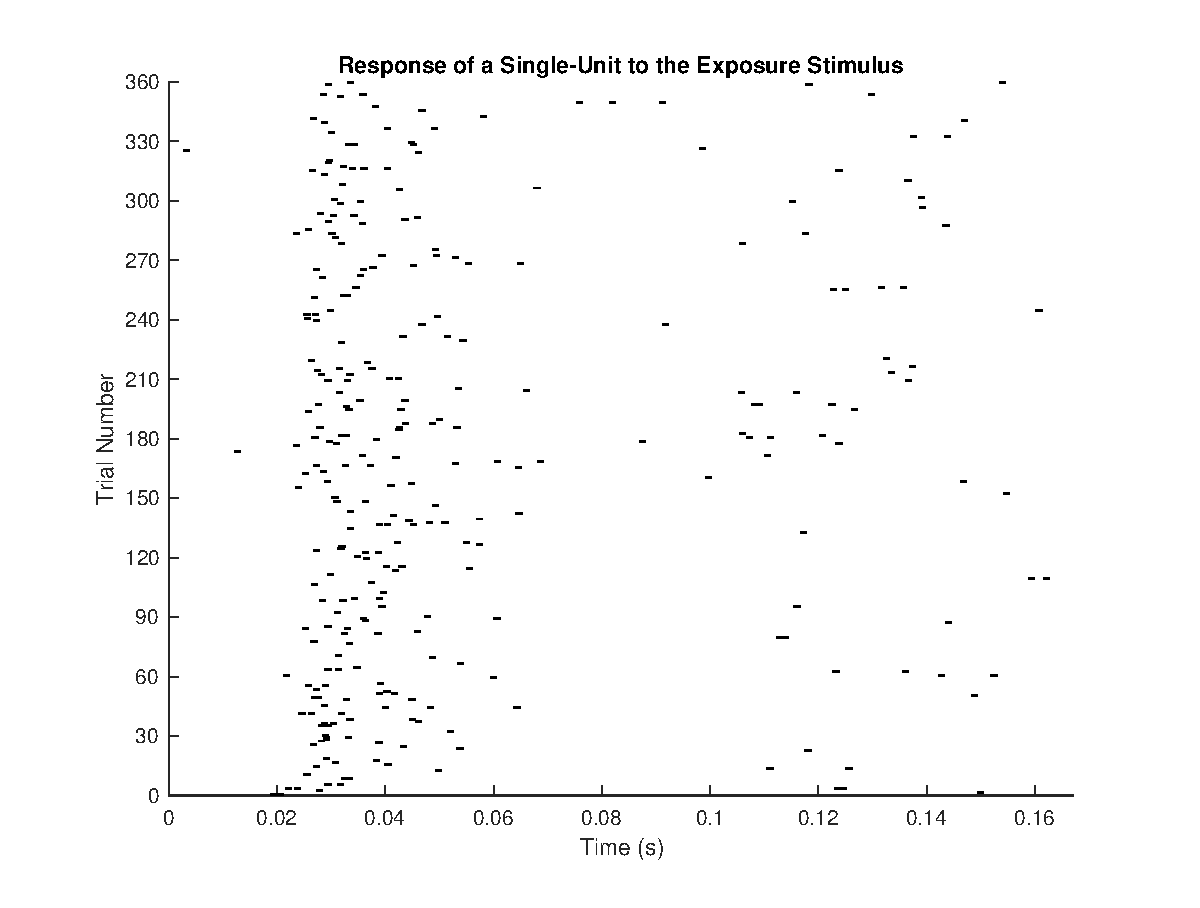
\includegraphics[width=1\textwidth]{RasterPlot.eps}
\caption{Raster Plot of Single-Unit Activity.}
\label{fig:RasterPlot}
\end{figure}

\subsection{Gaussian Kernel Firing Rate Estimate}

We calculate the estimate of the firing rate of this single-unit neuron by writing the following code:
\lstinputlisting[firstline=24, lastline=44]{exposure_stimulus_investigation.m}
This code simply places a Gaussian distribution with a standard deviation of 0.005s centered at the location of each spike and averages these distributions over all stimulus trials. This work produces Figure \ref{fig:Gaussian}, which shows that the firing rate increases dramatically around 0.03s into the trial, going from a baseline firing rate of about 5 Hz to a peak of just over 25 Hz.

\begin{figure}[ht!]
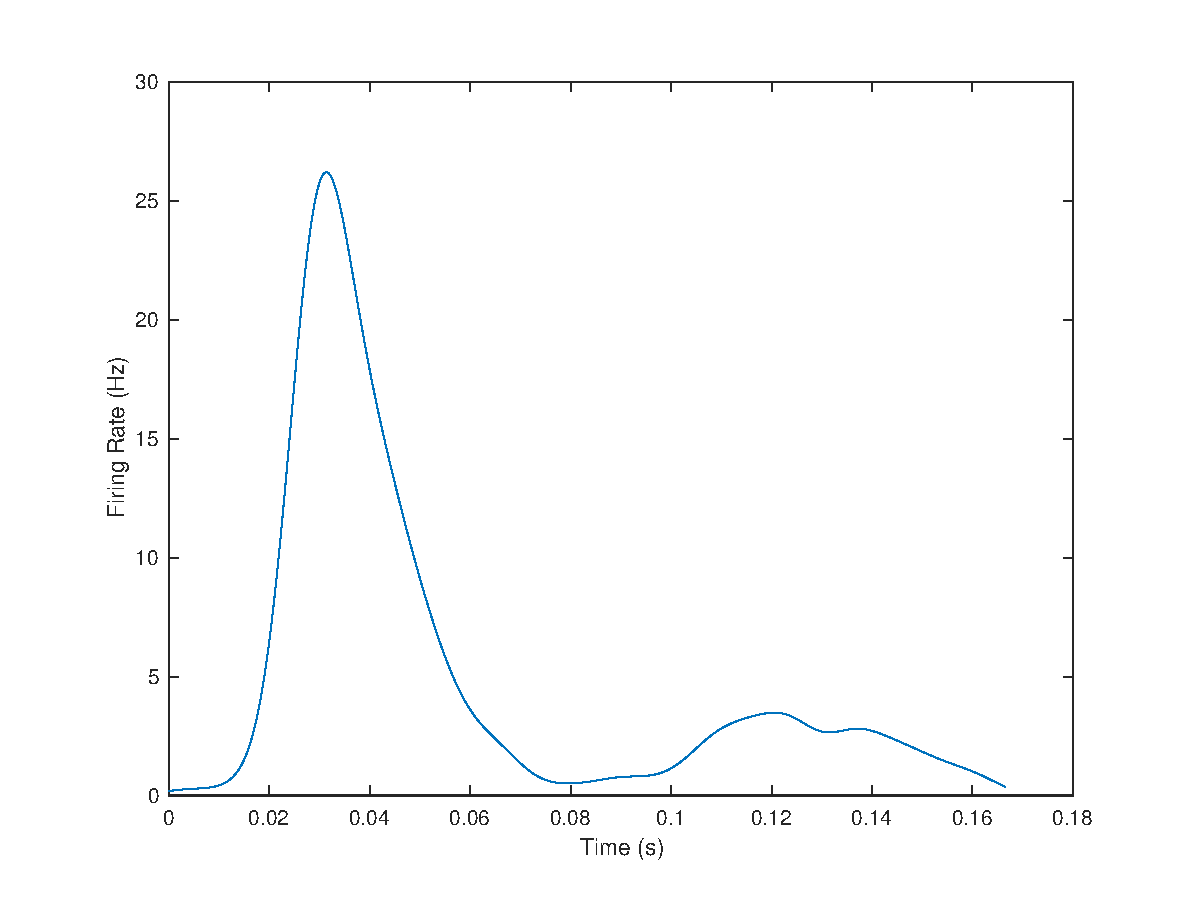
\includegraphics[width=1\textwidth]{fivemillisecondplot.eps}
\caption{Gaussian Estimation of Firing Rate Using $\sigma = 0.005s$.}
\label{fig:Gaussian}
\end{figure}

\subsection{Gaussian Kernel Parameter Variation}

We next alter the $\sigma$ parameter of the Gaussian kernel from above and generate Figures \ref{fig:point5ms} and \ref{fig:50ms} which shows the effect of this change. We used the following code to make these figures.
\lstinputlisting[firstline=46, lastline=68]{exposure_stimulus_investigation.m}
We can see from these figures that a very small standard deviation results in a quite noisy curve with large, quick oscillations, which intuitively, does not seem to describe the behavior of the neuron well as it is unlikely the firing rate would change that quickly. Conversely, a very large standard deviation results in a very smooth, wide curve that also does not seem to describe the data well as it predicts a large firing rate at the start of the experiment, where the raster plot indicates there is very little activity.

\begin{figure}[ht!]
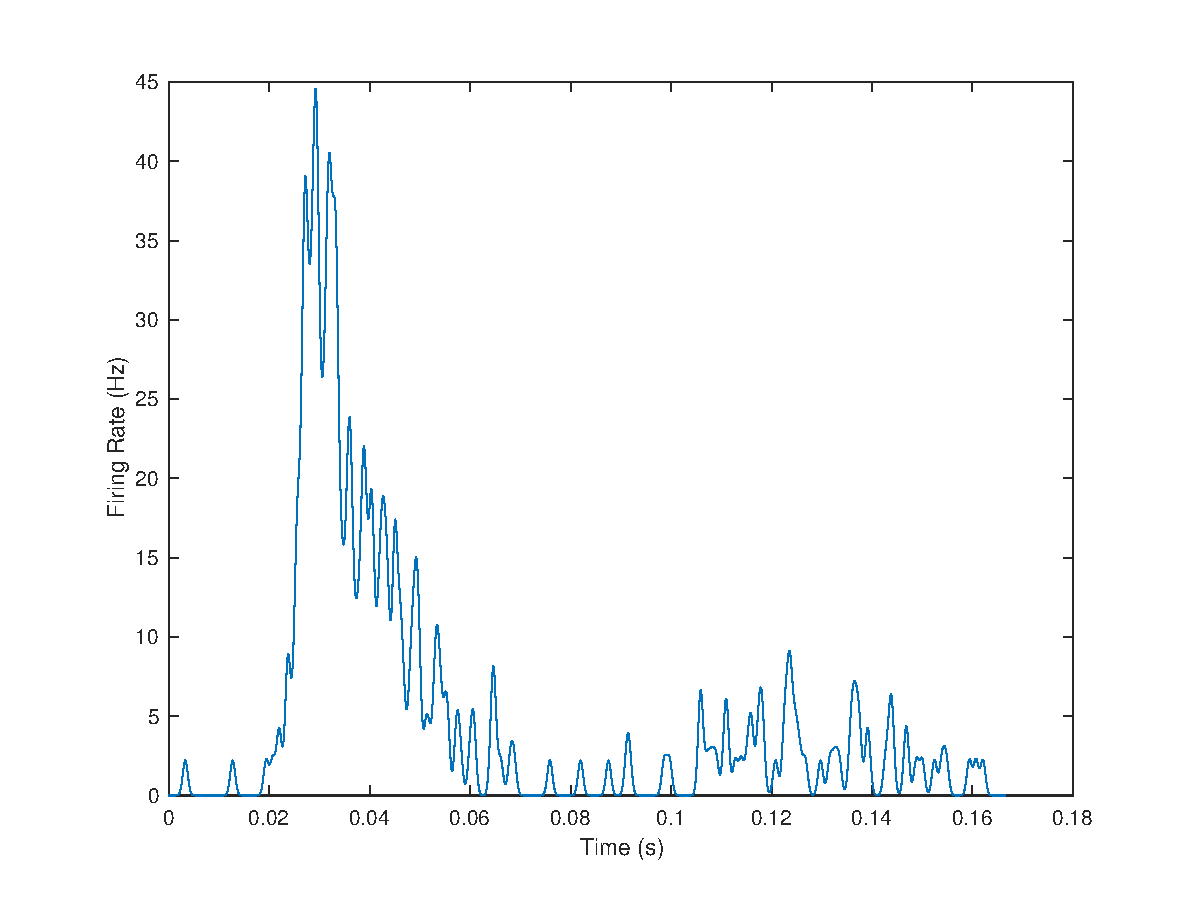
\includegraphics[width=1\textwidth]{halfmillisecondplot.eps}
\caption{Gaussian Estimation of Firing Rate Using $\sigma = 0.0005s$.}
\label{fig:point5ms}
\end{figure}


\begin{figure}[ht!]
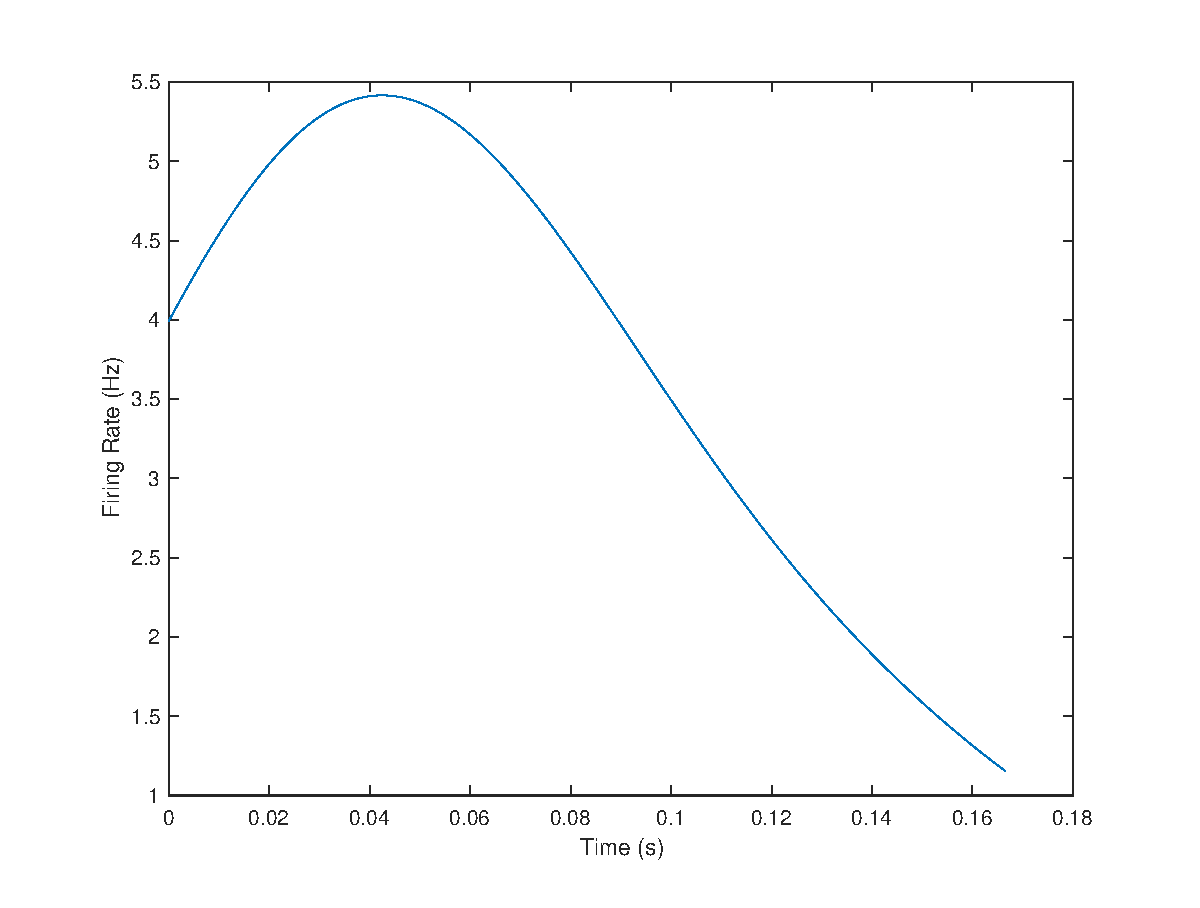
\includegraphics[width=1\textwidth]{fiftymillisecondplot.eps}
\caption{Gaussian Estimation of Firing Rate Using $\sigma = 0.05s$.}
\label{fig:50ms}
\end{figure}

\subsection{Grand Average Post-Stimulus Time Histogram}
We compute the grand average poststimulus time histogram using the following code:
\lstinputlisting[firstline=70, lastline=87]{exposure_stimulus_investigation.m}
This code generates Figure \ref{fig:PSTH}, which shows us the same trend we saw in the previous figures. The stimulus evokes a larger response from the population of neurons about 0.03 seconds after the onset of a trial.

\begin{figure}[ht!]
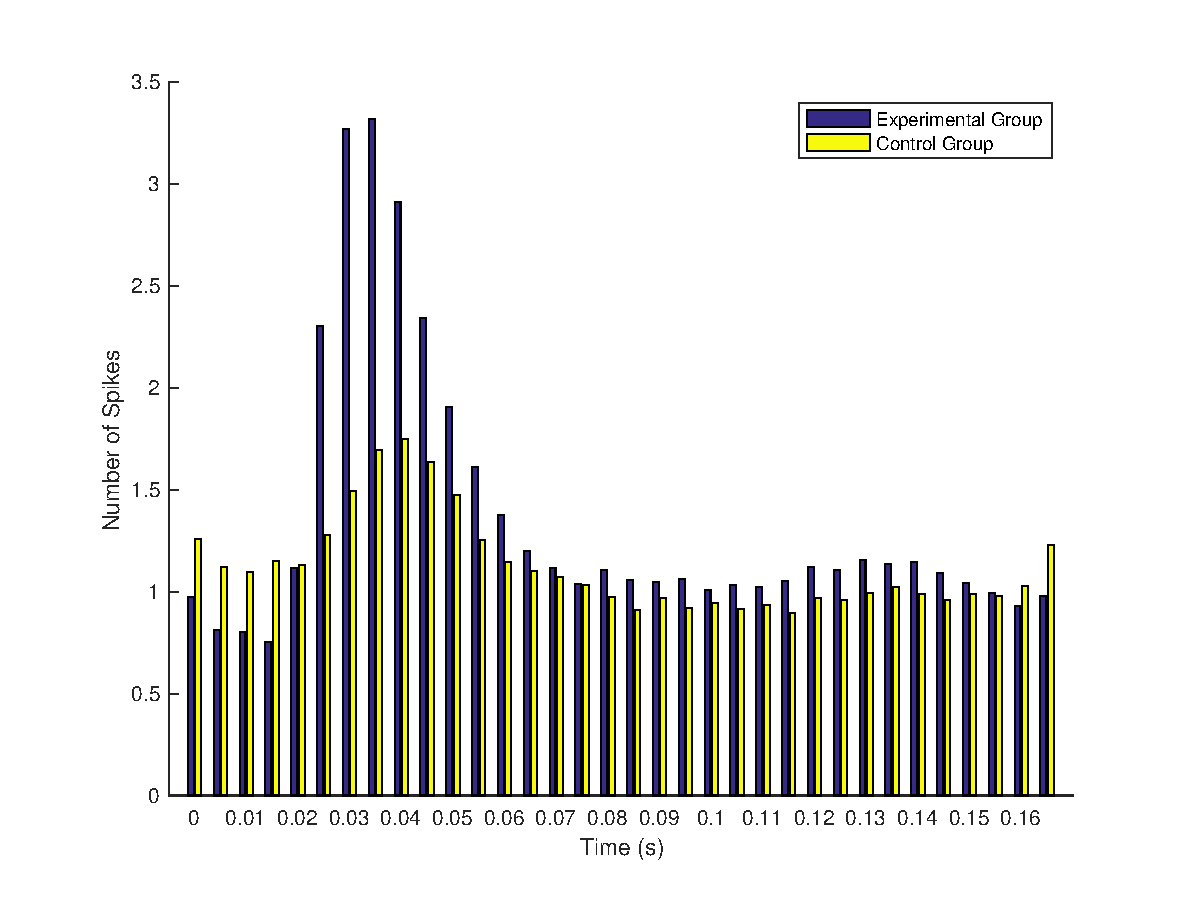
\includegraphics[width=1\textwidth]{Q1PD.eps}
\caption{Grand Average Post-Stimulus Time Histogram of two Populations of Neurons. Bin width was 5ms.}
\label{fig:PSTH}
\end{figure}

\subsection{Differences between Experimental and Control Groups}

Looking at Figure \ref{fig:PSTH}, we see that the experimental group has a stronger response (i.e. more spikes)
during the peak firing activity (about 0.02s to 0.05s after the onset of the trial) of the neurons. However, the control neuron population still exhibits this increase, so therefore it is just that the experimental group of neurons became more selective to the exposure stimulus while the precision of the response did not appear to change. Finally, we can see that there is very little difference in the activity of the two groups (beyond some higher activity in the control group at the start and end of a trial) outside of this peak firing range.

\subsection{Spike-Triggered Average for Neuron}

We generate a spike-triggered average using the following code:
\lstinputlisting[firstline=1, lastline=29]{sta_estimation.m}

This code generates Figure \ref{fig:sta_spectro}, which plots the spike-triggered average spectrogram from the DMR stimulus.

\begin{figure}[ht!]
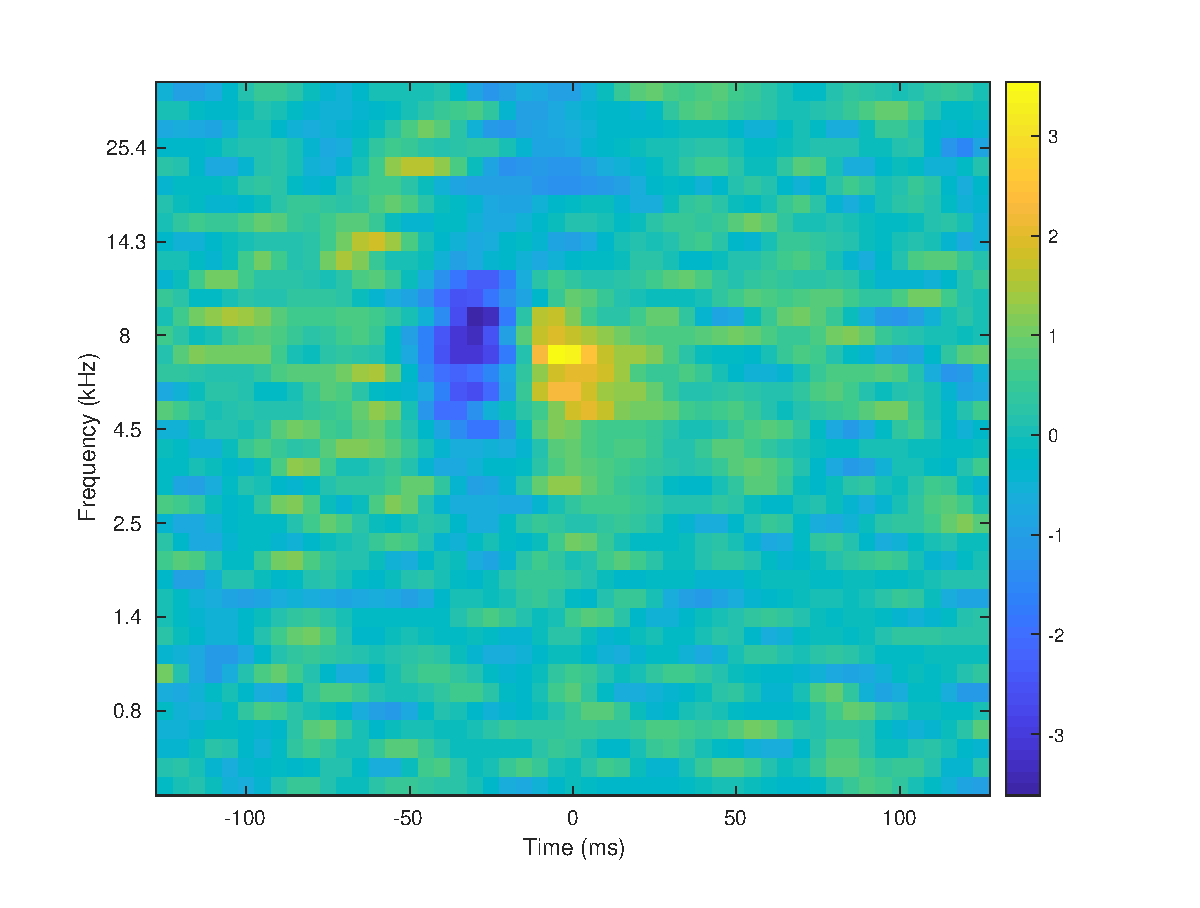
\includegraphics[width=1\textwidth]{sta_spectro.eps}
\caption{Spectrogram of spike-triggered average from DMR stimulus. Time range: $\pm$ 125 ms.}
\label{fig:sta_spectro}
\end{figure}

\subsection{Frequency Selectivity of Neuron}

The neuron appears to be most sensitive to a frequency of 7127 Hz.

\subsection{Neuronal Stimulus Preference}

According to the STA, the neuron's peak response would be higher to a brief tone pip. This is because if the neurons were responsive to constant tones, we would expect longer stretches of spikes instead of short bursts. The tone pip should be about 30ms long to evoke the largest response.

\subsection{Potential Stimulus Correlations}

We plot the stimulus correlation matrix using the following code:
\lstinputlisting[firstline=31, lastline=34]{sta_estimation.m}
This code generates Figure \ref{fig:stim_corr}, which appears to be close to an identity matrix.

\begin{figure}[ht!]
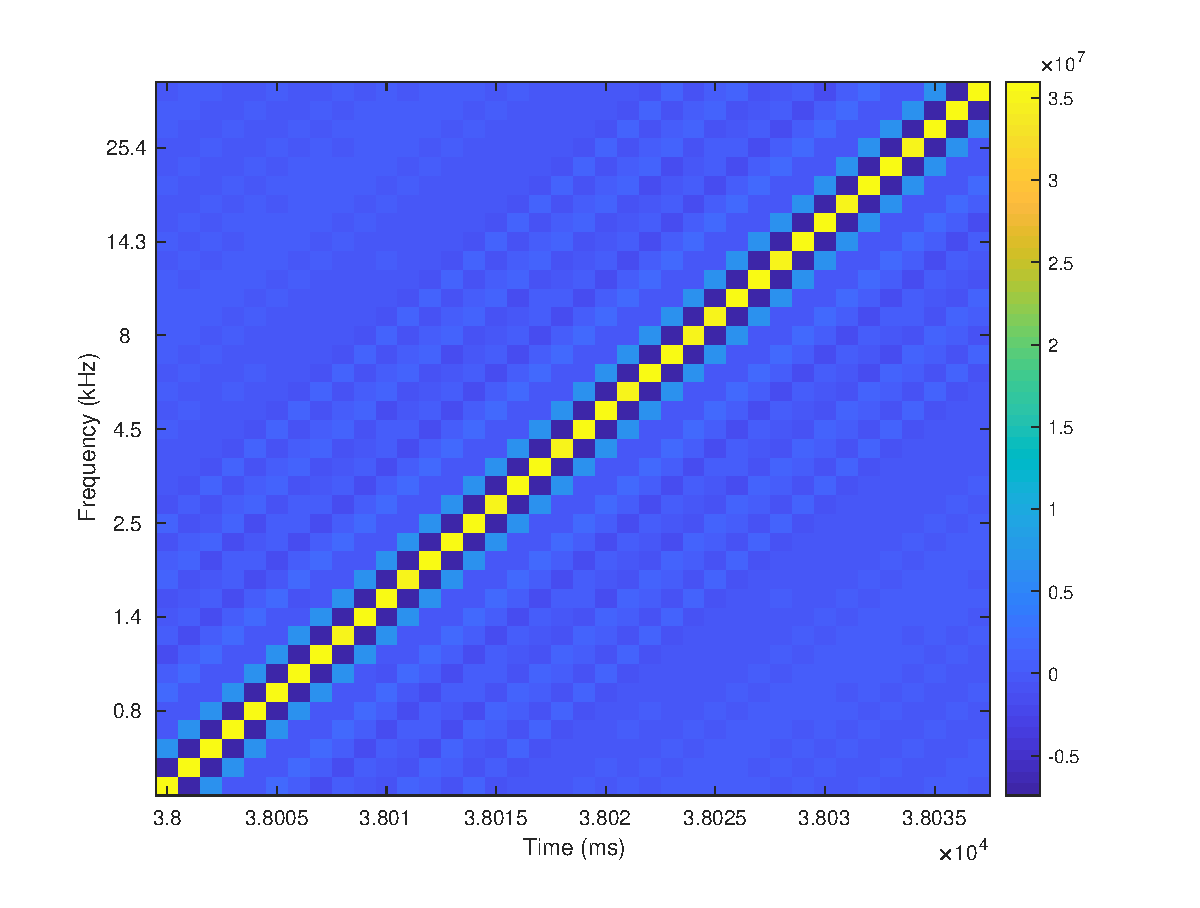
\includegraphics[width=1\textwidth]{stimulus_correlation.eps}
\caption{Spectrogram of stimulus correlation matrix.}
\label{fig:stim_corr}
\end{figure}


\section{Random Neural Networks and Overfitting in Regression}

\subsection{Linear Regression with Regularization}

We implement linear regression with regularization in Matlab as follows:
\lstinputlisting[firstline=1, lastline=59]{nn_regression.m}
This produces Figure \ref{fig:regression} which shows us how this network performs on test data. We see from this data that the 26 neuron model performed the best (as measured by mean squared error and visual inspection of the curve it makes), while the 10 neuron model performed reasonably well, but with some more error. Finally, the 2 neuron model performed the worst of all and has quite the large error.

\begin{figure}[ht!]
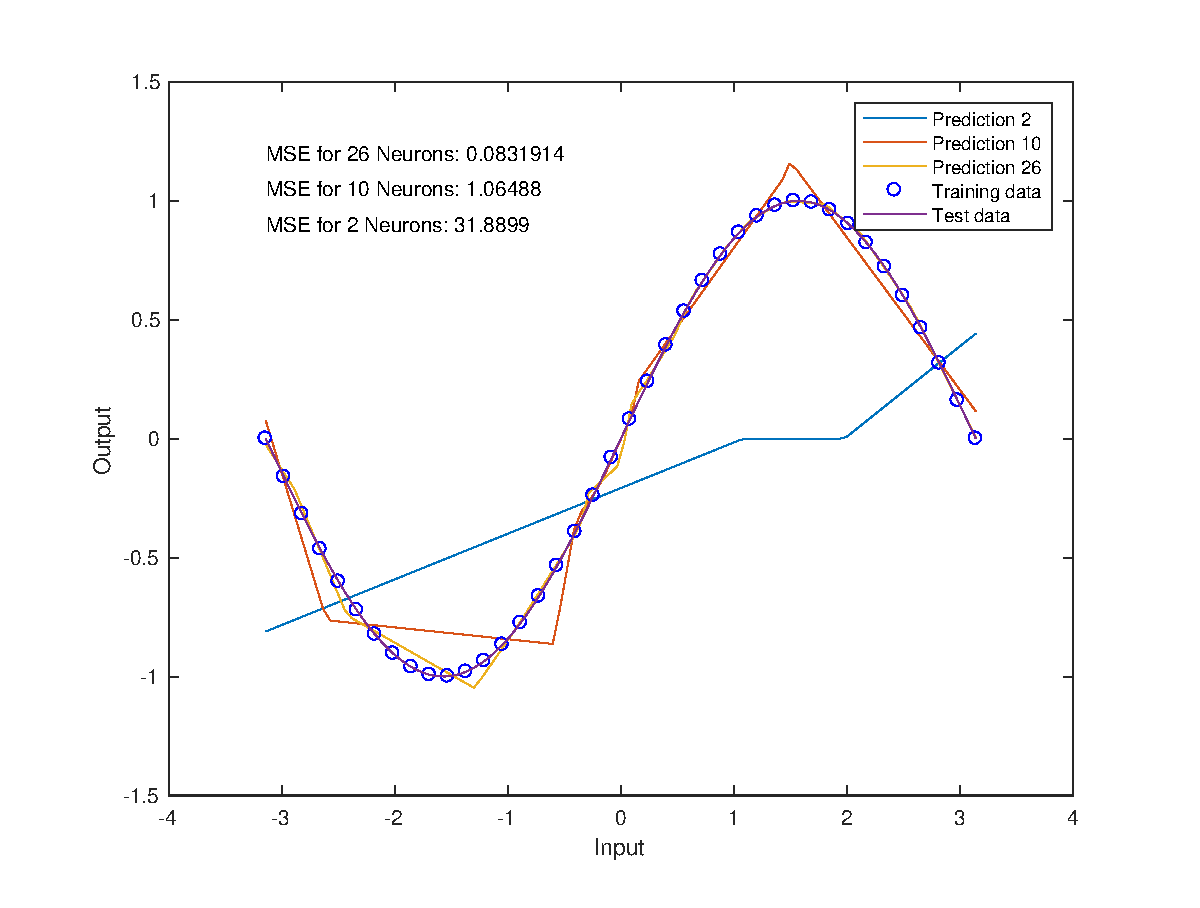
\includegraphics[width=1\textwidth]{Q2PartA.eps}
\caption{Performance of Simple Linear Regression with varying numbers of neurons}
\label{fig:regression}
\end{figure}

\subsection{Overdetermined Networks}

We implement the overdetermined network scenario as follows:
\lstinputlisting[firstline=61, lastline=108]{nn_regression.m}
This code produces Figure \ref{fig:overdetermined}, which shows us what happens in the overdetermined network scenario. We see from this figure that the network is quite unstable throughout this size range. Indeed, the mean squared error is quite low for networks with less than 10 neurons, 15 neurons, or 25 neurons. However, the mean squared error is astronomically high for values close to this: networks with 12, 21, and 22 neurons. Thus, we see that when the model is too small, the mean squared error might be low, but the predictions don't map neatly onto the ``ideal'' function we are approximating (as seen in Figure \ref{fig:regression}). However, when the model is too big, the mean squared error is quite large and the model likely fits the data too well such that it cannot generalize to new test data.

\begin{figure}[ht!]
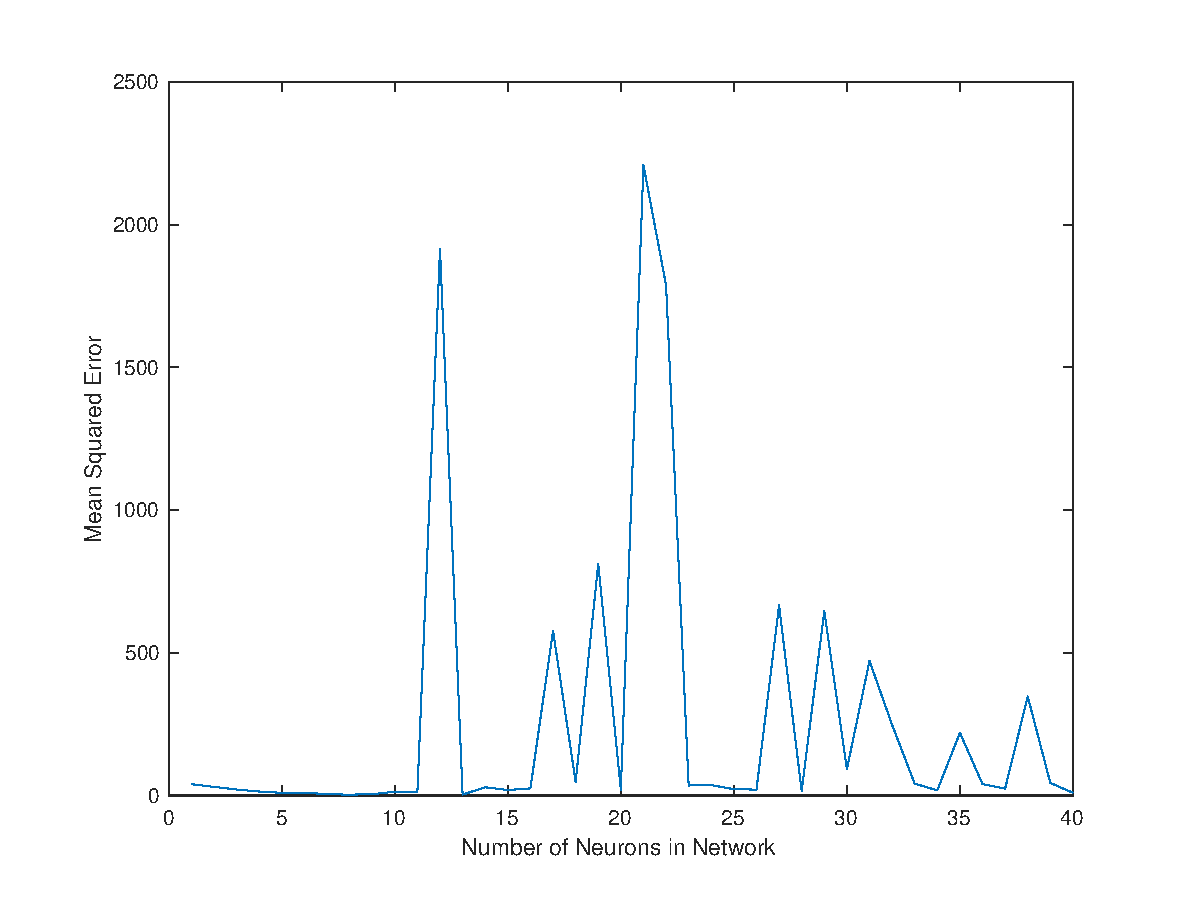
\includegraphics[width=1\textwidth]{Q2PartB.eps}
\caption{Mean-Squared Error as a Function of Network Size for the Over-Determined Situation.}
\label{fig:overdetermined}
\end{figure}

\subsection{Underdetermined Networks}

We implement the underdetermined network scenario as follows:
\lstinputlisting[firstline=110, lastline=157]{nn_regression.m}
This code produces Figure \ref{fig:underdetermined}, which we see produces a low mean-squared error for large network sizes. Thus, based on this figure, we would guess that the best network size is approximately 110 neurons or so (as the mean squared error seems to plateau after this). The performance of these big networks is not as variable as the smaller networks.

\begin{figure}[ht!]
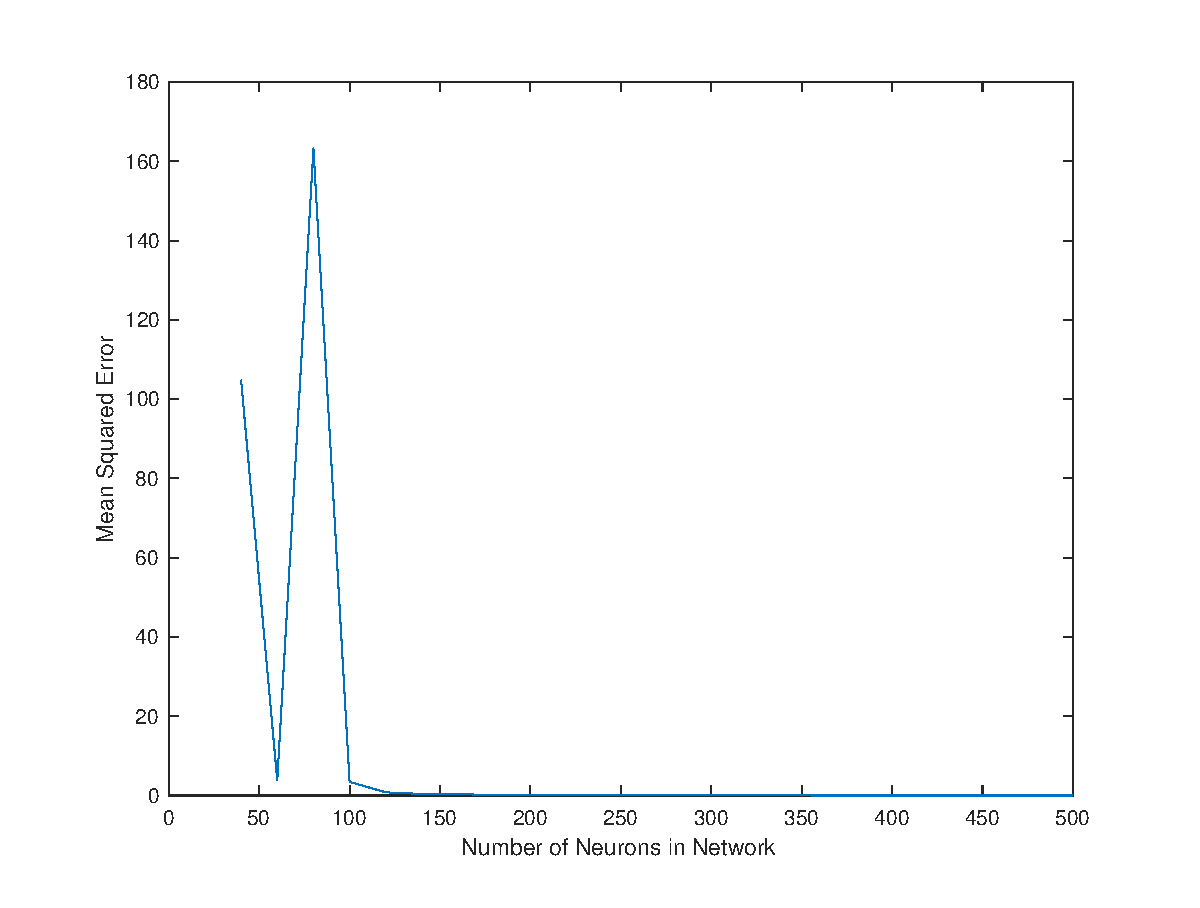
\includegraphics[width=1\textwidth]{Q2PartC.eps}
\caption{Mean-Squared Error as a Function of Network Size for the Under-Determined Situation.}
\label{fig:underdetermined}
\end{figure}

\subsection{Label Noise and Regularization Parameters}

We implement these models as follows:
\lstinputlisting[firstline=159, lastline=298]{nn_regression.m}
This produces Figure \ref{fig:noiseAndReg}

\begin{figure}[ht!]
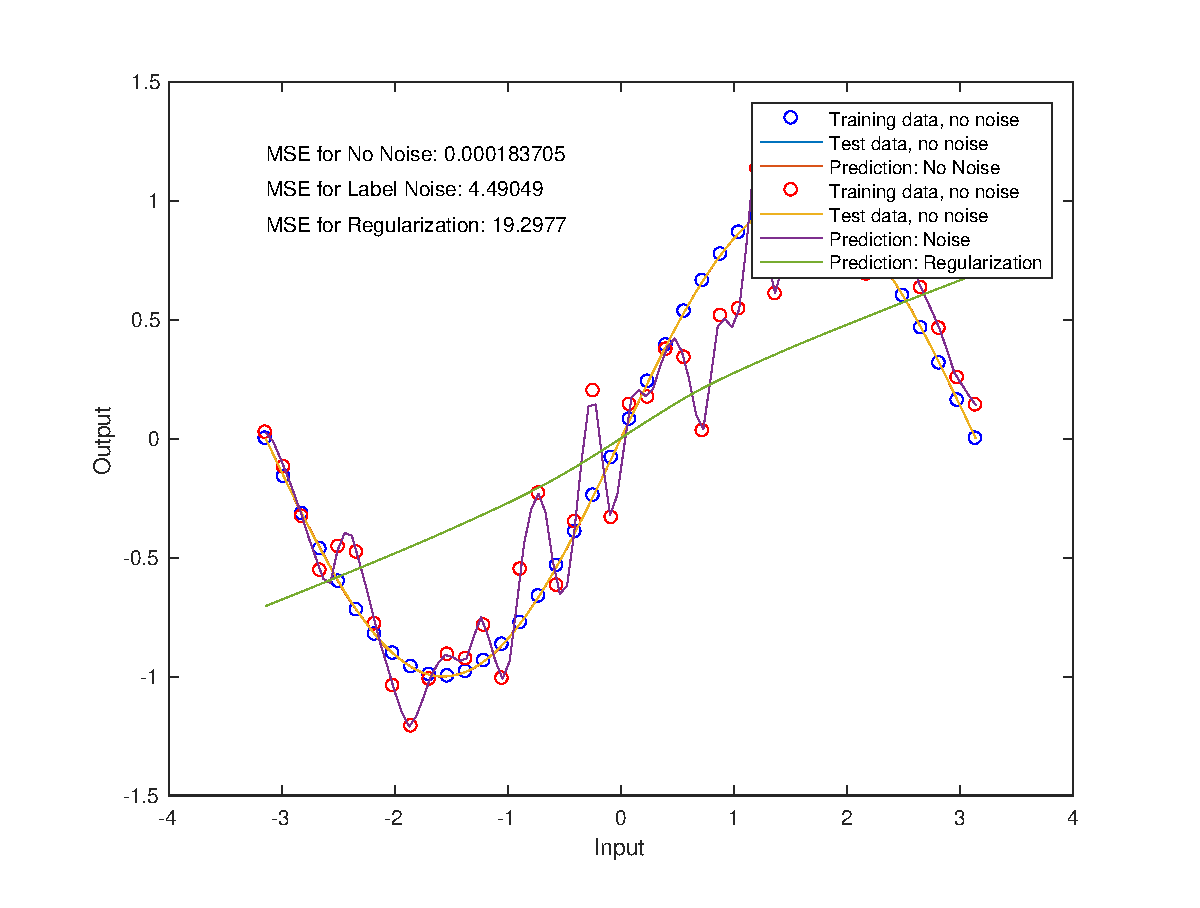
\includegraphics[width=1\textwidth]{Q2PartD.eps}
\caption{Performance of Linear Regression Neural Networks When Labels Contain Noise and Regularization is Used.}
\label{fig:noiseAndReg}
\end{figure}

We see from the figure that the typical mean squared error for the model without noise is quite low for a neural network this size (on the order of $10^{-4}$). However, when there is label noise, the mean squared error is higher (on the order of 0-10). Thus, we can see that introducing noise potentially disturbs a large, overfitted network by several orders of magnitude. The predictions with label noise look good, in that they almost always hit the labels, but we can see that this model does not do a good job approximating the true, underlying function buried in the noise, which makes the model as a whole not that good. The regularization parameter increases the mean squared error for the system without noise (as seen in the figure). However, for the model with noise, this regularization would make it a better model and reduce the overfitting problem for a value of $\lambda$ that is reasonable (though in this example, the regularization is too strong and makes it a poor model).

\subsection{Reflections}

Based on these results, it makes some sense for neural networks to massively expand the dimensions, as neural networks with large dimensions are more stable and potentially provide better accuracy and generalization. However, this must be done carefully, as the data is likely noisy and we must avoid overfitting the data. This can be done with networks of large dimensions by providing an appropriate regularization parameter. Thus, with this addition, networks of larger dimension will likely be quite suitable for use and application. We would argue that the regime that is most relevant to the learning problems faced by the brain is the one with noise (as neurons are quite noisy and neurons are likely a part of other networks that provide activity that may be irrelevant to the task of interest). Further, the brain likely faces an underdetermined regime (where there are fewer training samples than parameters) as the brain contains billions of neurons, and even if a fraction of these are involved in any one computation, this still comprises a huge number of parameters to tune relevant to the data a brain could receive.

\section{Image Demixing}

\subsection{Covariance Matrix and PCA}

\subsubsection{De-meaning the data}

We write the following Matlab function to remove the mean from a data matrix:
\lstinputlisting[firstline=62, lastline=65]{problem3code/problem3.m}
We then check this code using the built in mean function in Matlab to ensure that it works as expected. This code is shown below:
\lstinputlisting[firstline=1, lastline=7]{problem3code/problem3.m}
This code returns a value of 0 (or very close to 0, which occurs due to rounding error and floating-point imprecision) for each column of the matrix as expected.

\subsubsection{Covariance Matrix Function}

We then computed the covariance matrix by creating the custom function below:
\lstinputlisting[firstline=67, lastline=69]{problem3code/problem3.m}
We then tested this code with the following, which showed us that this covariance function works the same as the in-built function:
\lstinputlisting[firstline=9, lastline=11]{problem3code/problem3.m}


\subsubsection{Eigenvectors and values of covariance matrix}

We use the built-in eig function in Matlab to calculate the principal components (code shown below), which are shown on Figure \ref{fig:PCs}. Note that the PCs are each magnified by 5 times so we can see how they overlay on the data (as the direction, not the magnitude, of the PCs are important for this section).
\lstinputlisting[firstline=13, lastline=17]{problem3code/problem3.m}

\begin{figure}[ht!]
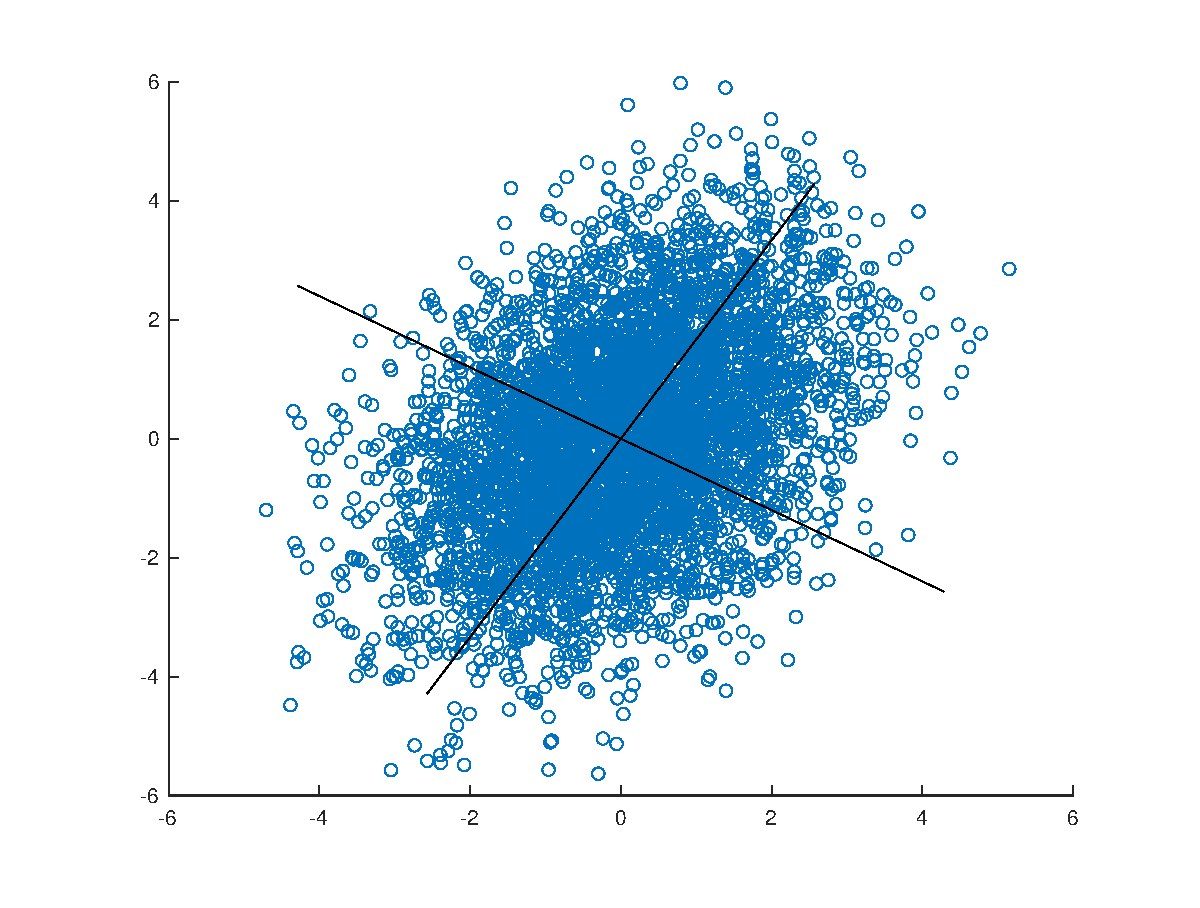
\includegraphics[width=1\textwidth]{pcs.eps}
\caption{The Principal Components of the toWhiten data overlaid on the data itself.}
\label{fig:PCs}
\end{figure}

\subsubsection{Time Required for Computation}

We can see that the covariance matrix is just a $2 \times 2$ matrix, so we can intuitively understand that the conditions leading to a long runtime for diagonalization of the covariance matrix will be data with large dimensions. That is, the runtime scales as a factor of the number of dimensions, D, not necessarily of the number of data points (as the number of data points is just used to calculate the covariance matrix, which is a fast operation). We can see this by running the following code on an early-2015 Macbook Pro with 8 GB RAM:
\lstinputlisting[firstline=19, lastline=39]{problem3code/problem3.m}
This gives us the following values for the various cases:

\begin{tabular}{|c|c|c|}
\hline
Type of Matrix & Covariance Method & SVD Method \\
\hline
$ 1000 \times 5000$ & 21.9225s &  3.6852s \\
\hline
$ 5000 \times 1000$ & 0.4502s & 3.0704s \\
\hline
\end{tabular}

As we can see from this, the SVD method, for large covariances matrices, is faster. Further, it confirms the above by showing us that a large covariance matrix increases the runtime.

\subsection{Whitening the Data}

We whitened the data as follows:
\lstinputlisting{problem3code/whiten_data.m}
We then tested this function on the toWhiten dataset, by running the following code:
\lstinputlisting[firstline=41, lastline=43]{problem3code/problem3.m}
This produces Figure \ref{fig:whitenedData}, which shows us that the data has been properly rotated or whitened.

\begin{figure}[ht!]
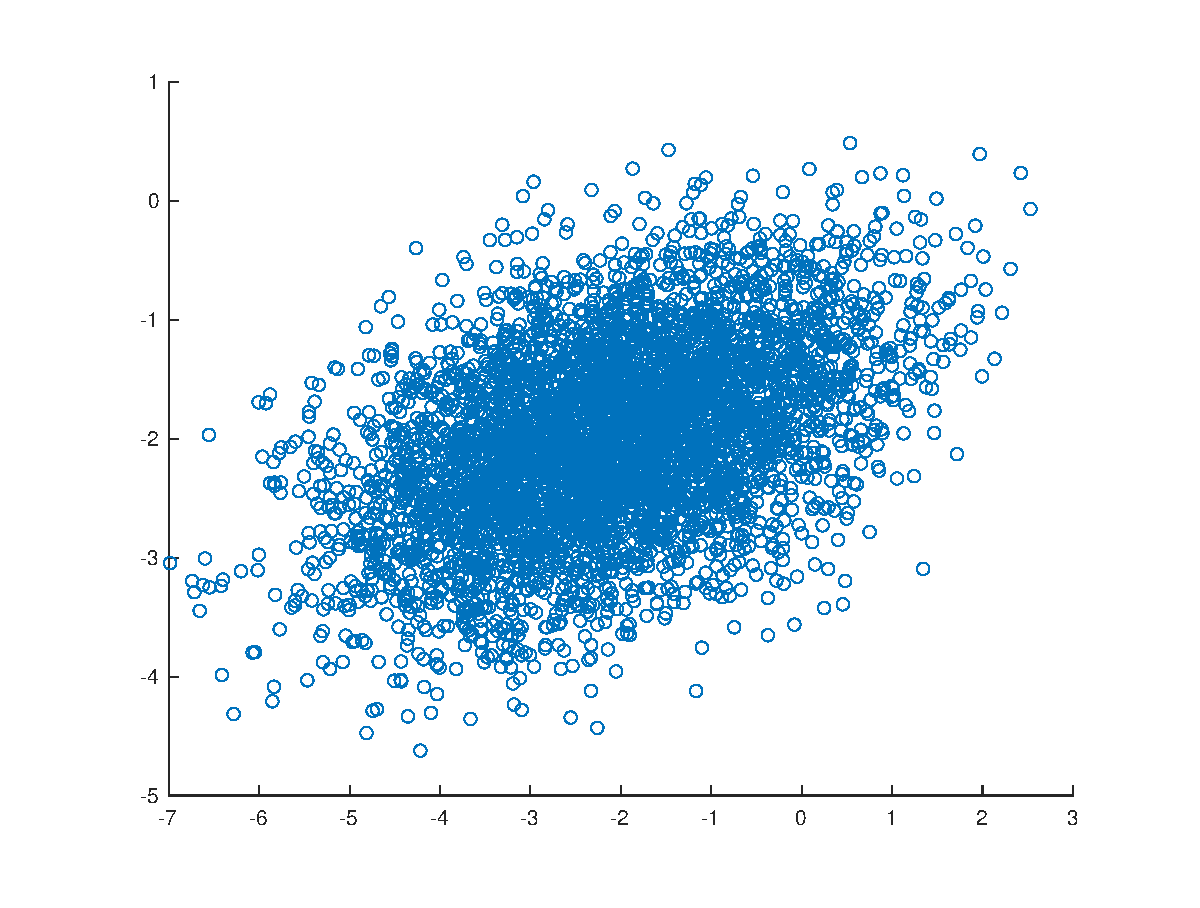
\includegraphics[width=1\textwidth]{whitenData.eps}
\caption{Whitened toWhiten Data.}
\label{fig:whitenedData}
\end{figure}

We can see from this that the principal components are now just the x and y axes, so to extract these from the whitened data, we need only take vectors that describe each axis (i.e. $(0, 1)$ and $(1, 0)$).


\subsection{ICA}

\subsubsection{Mixed Images}

We plotted the three images using the below commands:
\lstinputlisting[firstline=45, lastline=50]{problem3code/problem3.m}
This generates Figure \ref{fig:img1}, \ref{fig:img2}, and \ref{fig:img3}, which we can see look like forest scenes overlaid on one another.

\begin{figure}[ht!]
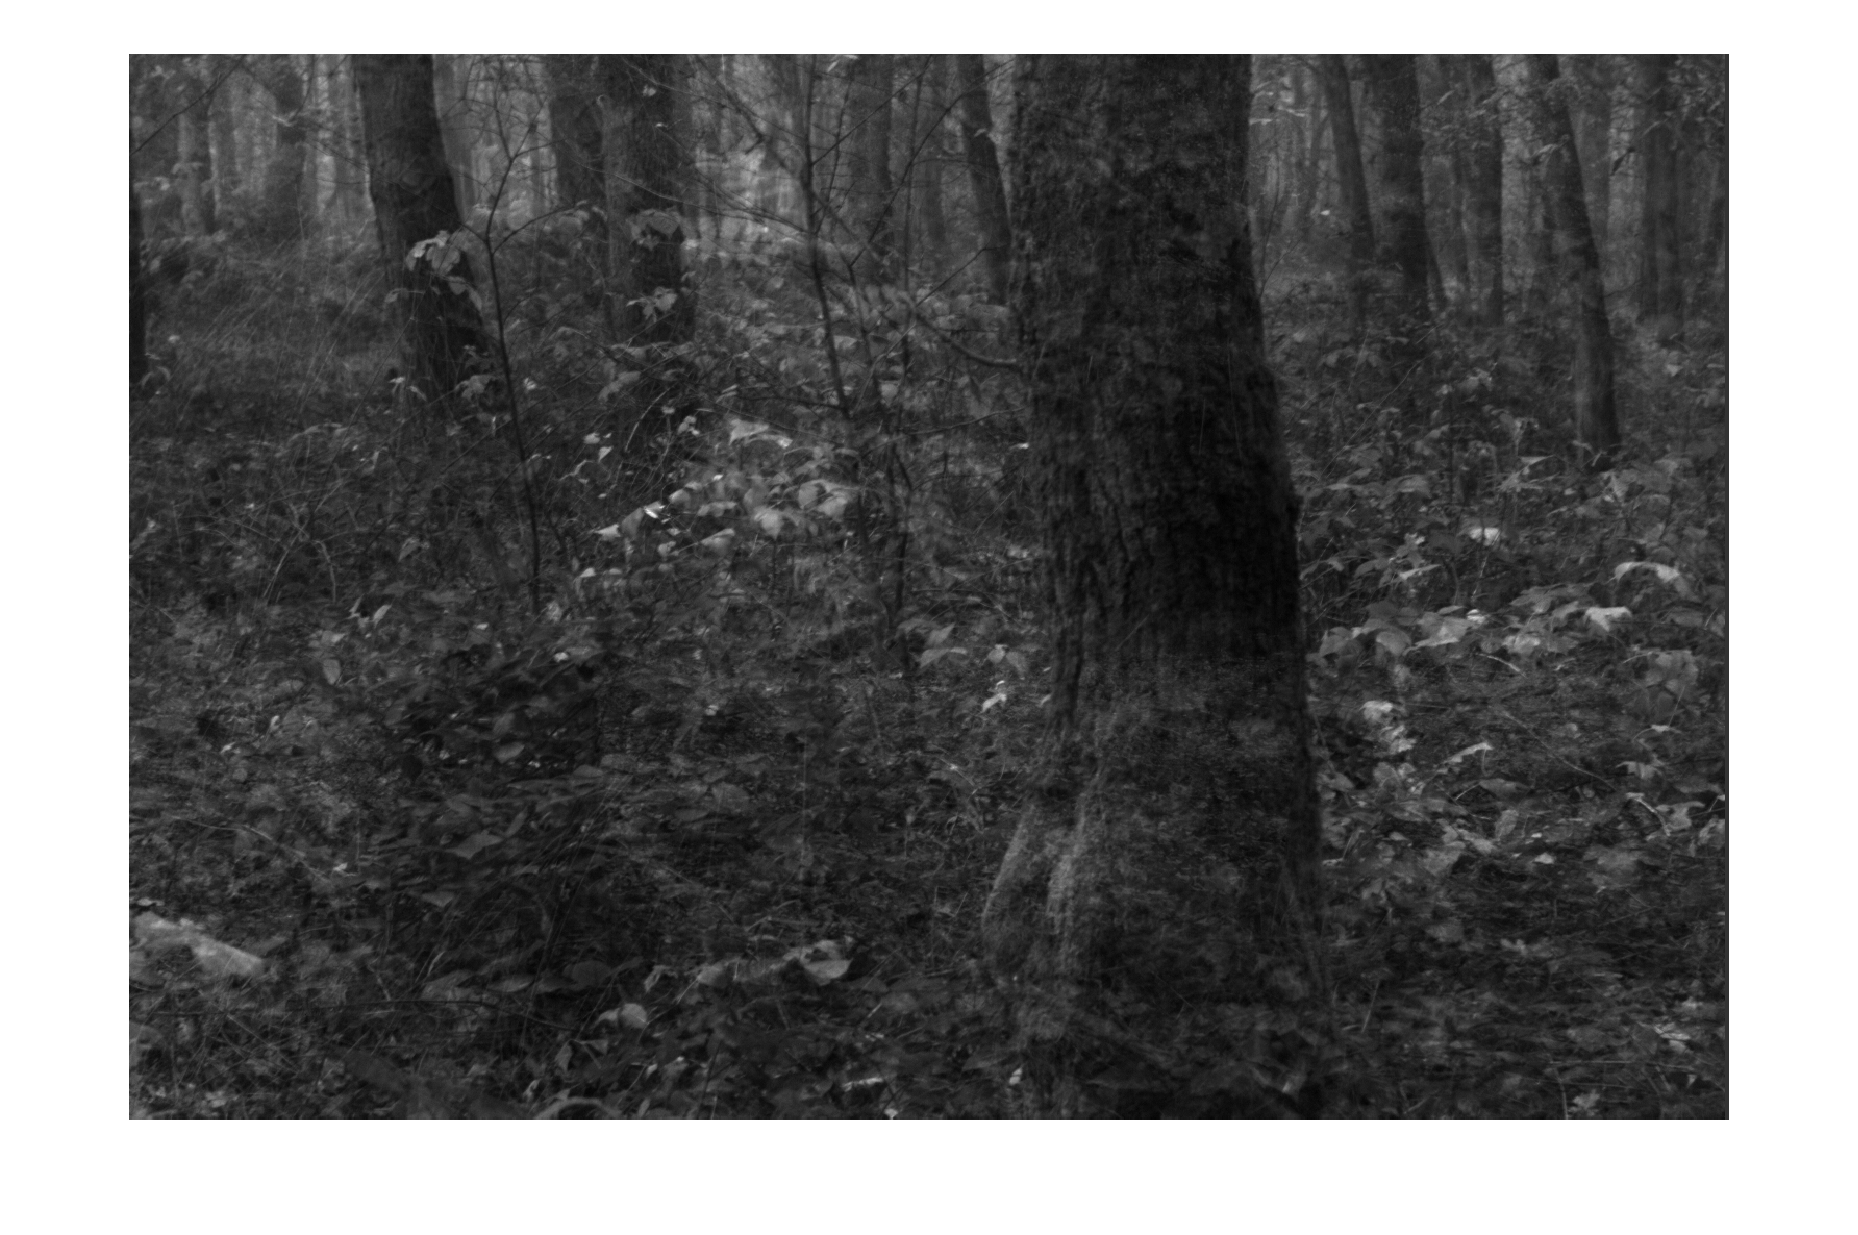
\includegraphics[width=1\textwidth]{img1.eps}
\caption{Unwhitened Version of Image 1}
\label{fig:img1}
\end{figure}

\begin{figure}[ht!]
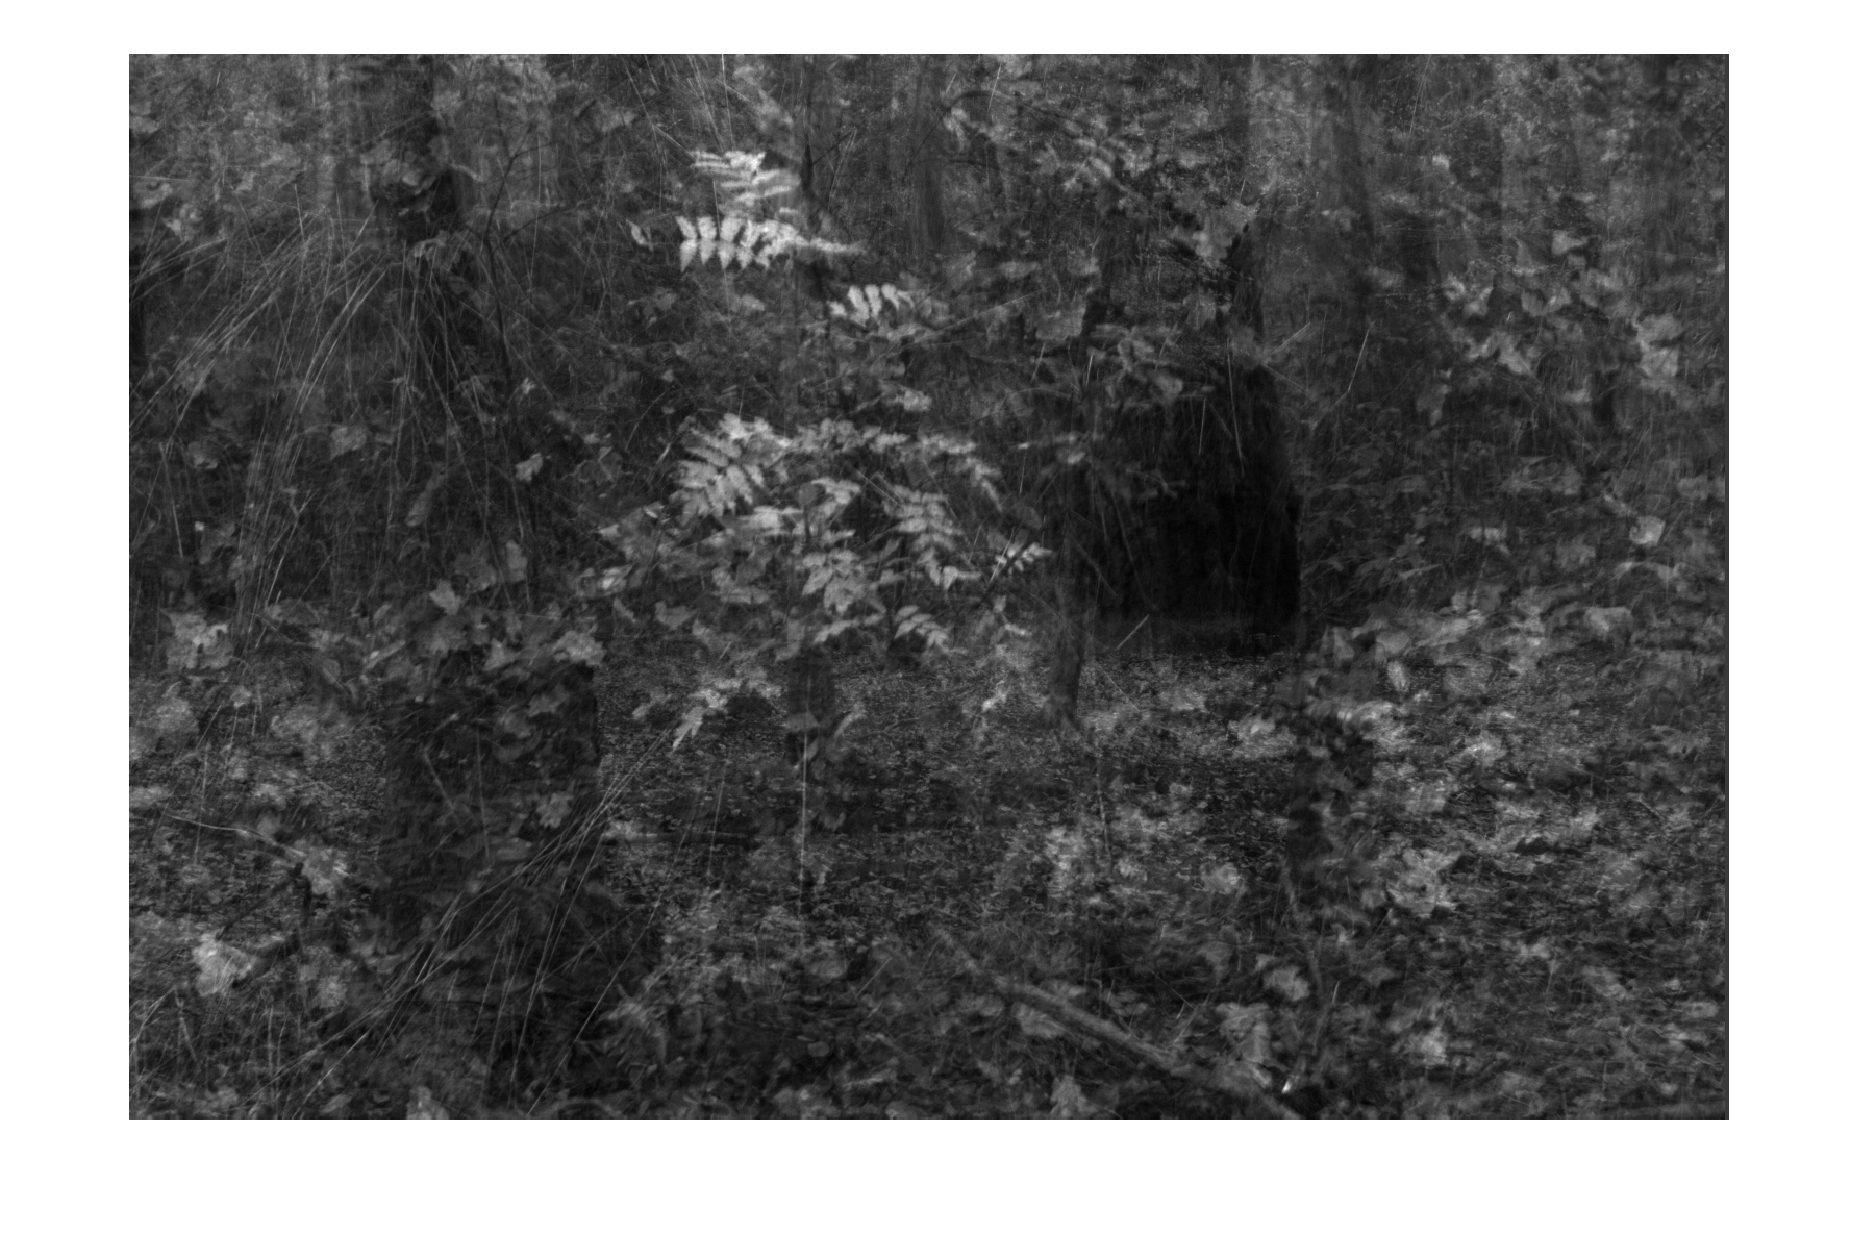
\includegraphics[width=1\textwidth]{img2.eps}
\caption{Unwhitened Version of Image 2}
\label{fig:img2}
\end{figure}

\begin{figure}[ht!]
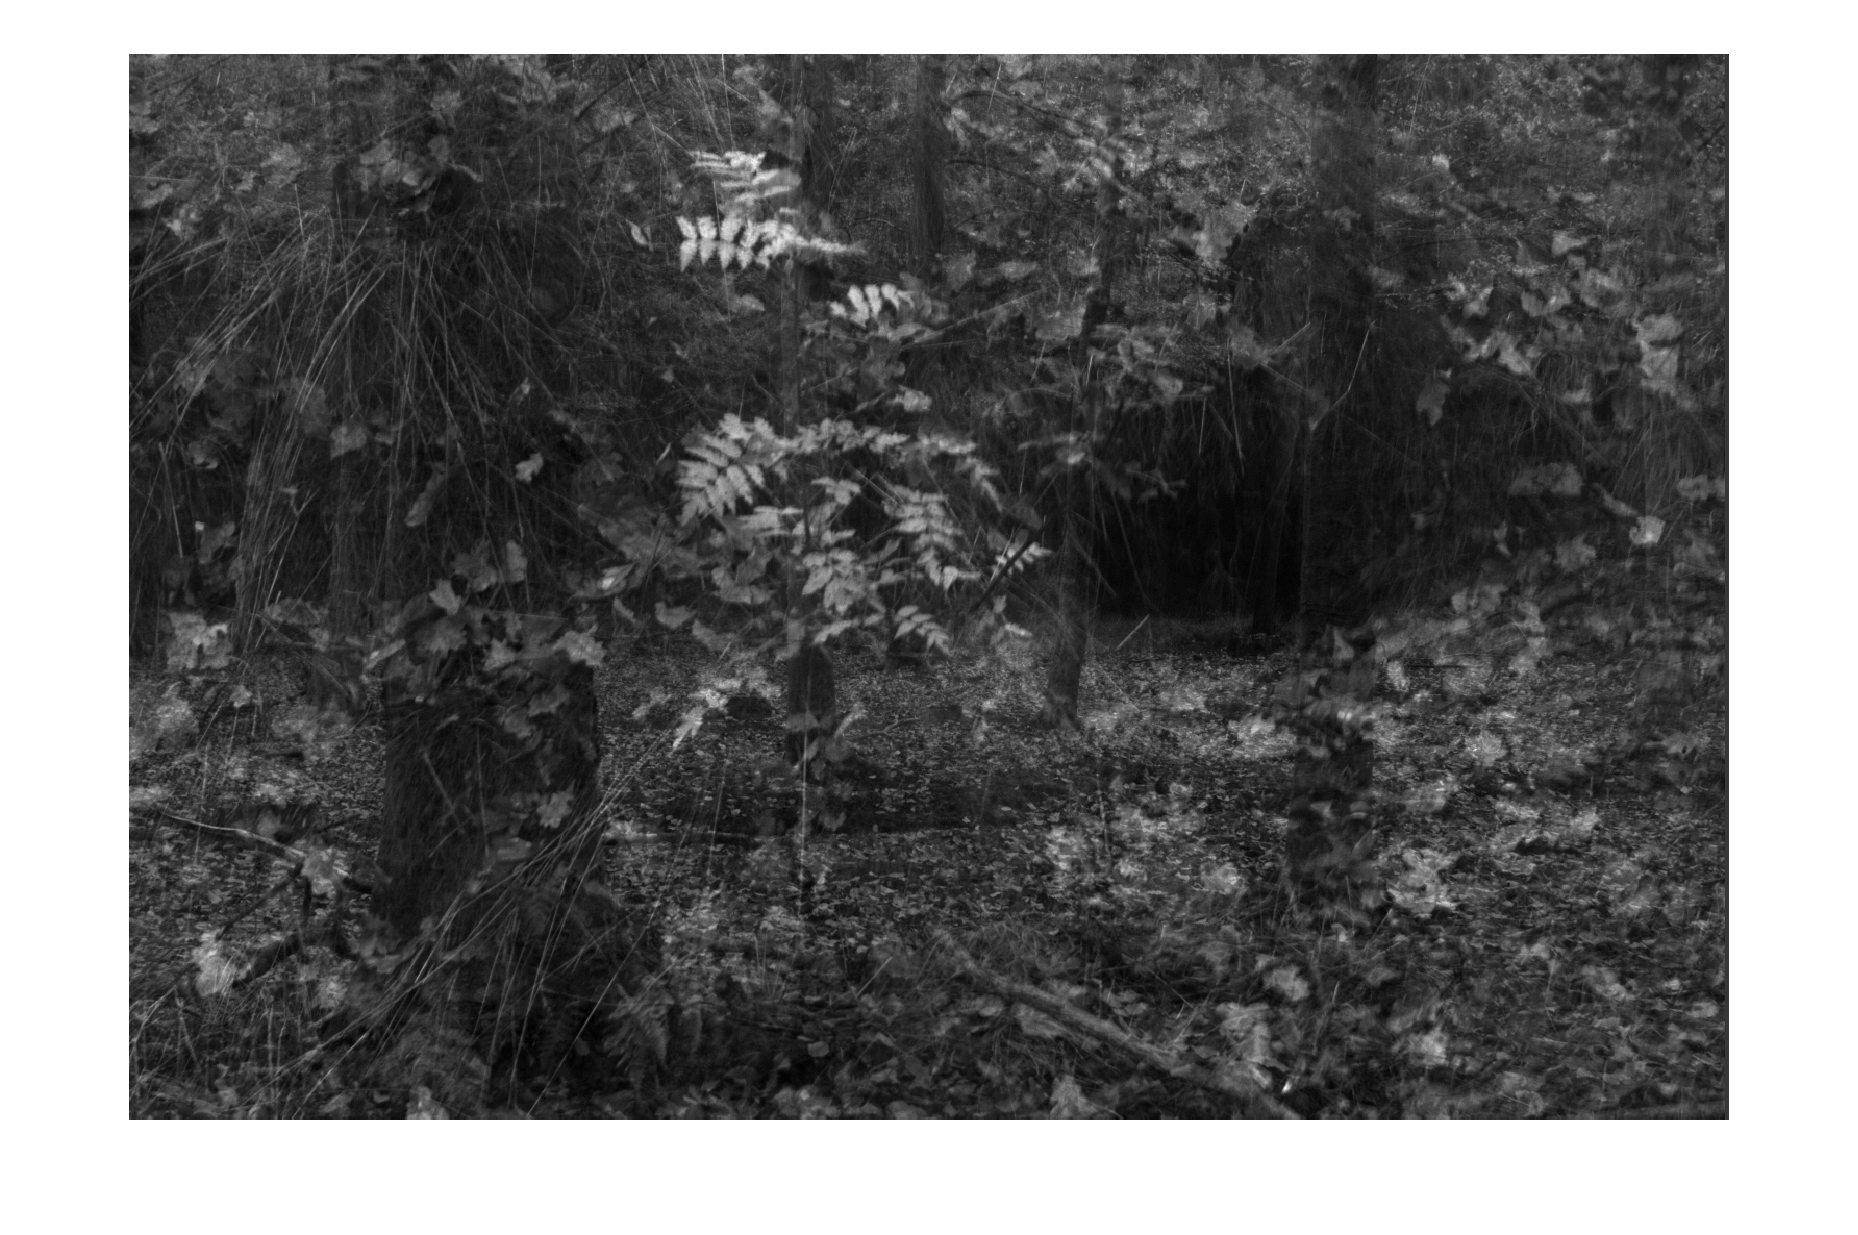
\includegraphics[width=1\textwidth]{img3.eps}
\caption{Unwhitened Version of Image 3}
\label{fig:img3}
\end{figure}

\subsubsection{Whitening mixed images}

We then whiten the images using the following code:
\lstinputlisting[firstline=52, lastline=54]{problem3code/problem3.m}
This produces the following whitened images shown in Figure \ref{fig:Wimg1}, \ref{fig:Wimg2}, and \ref{fig:Wimg3}.

\begin{figure}[ht!]
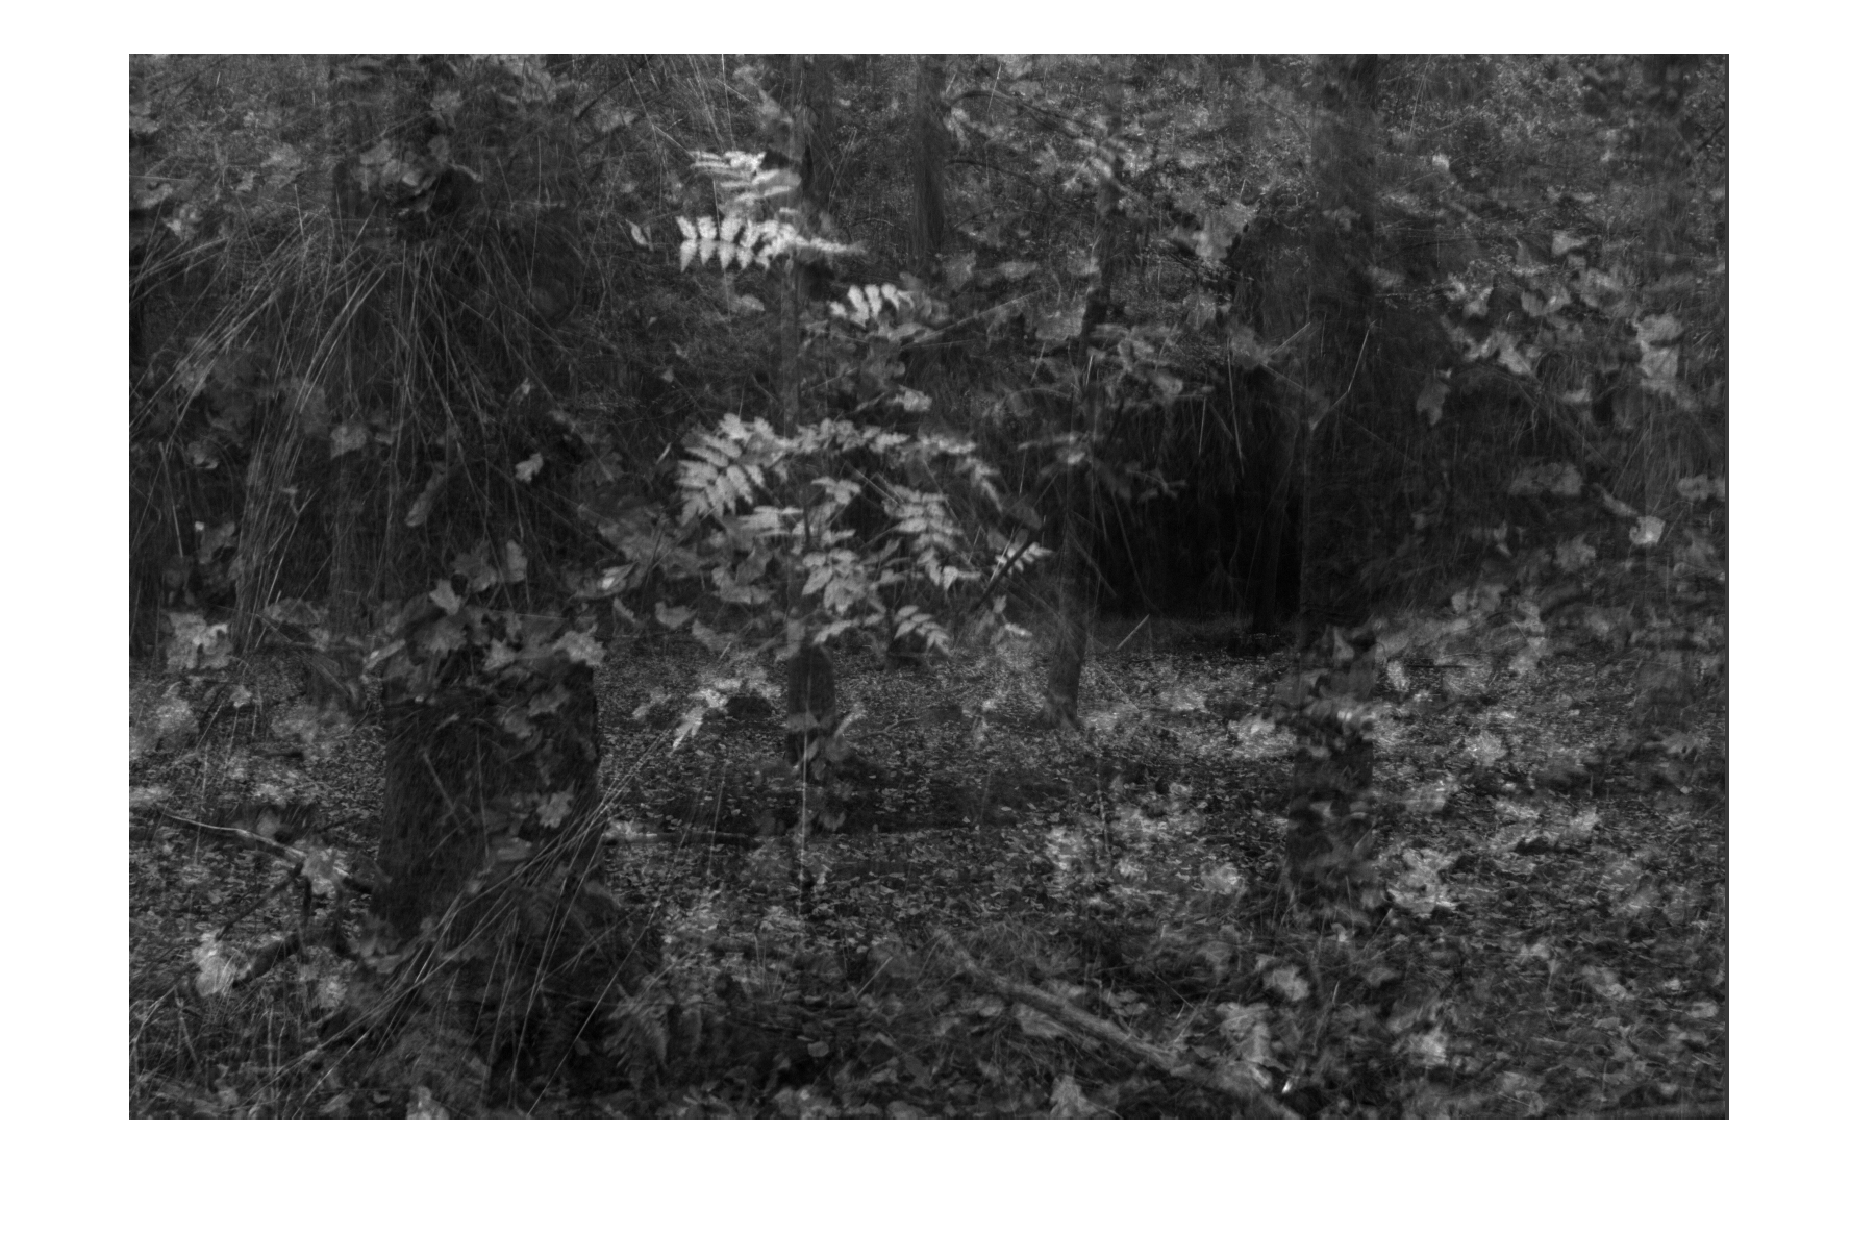
\includegraphics[width=1\textwidth]{Wimg1.eps}
\caption{Whitened Version of Image 1}
\label{fig:Wimg1}
\end{figure}

\begin{figure}[ht!]
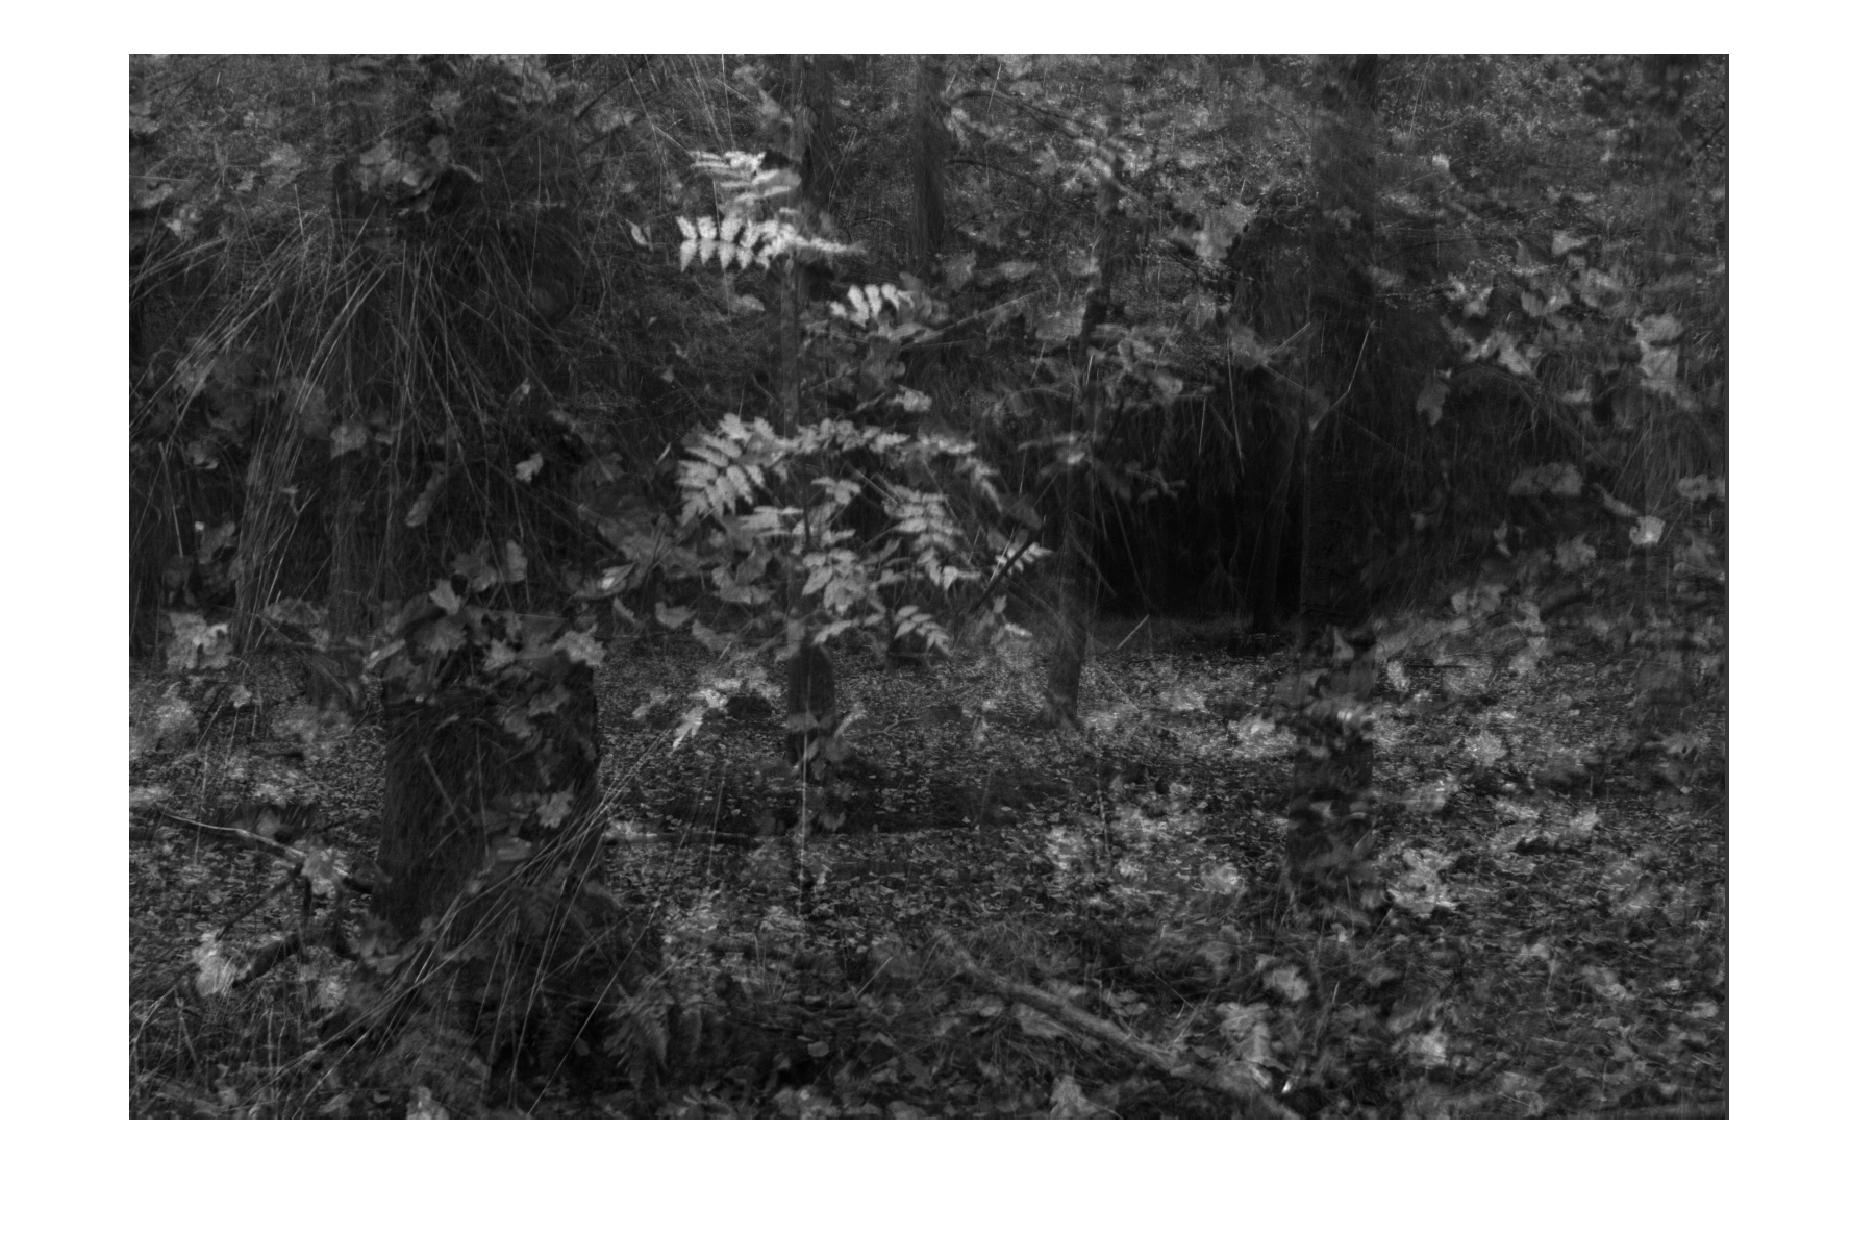
\includegraphics[width=1\textwidth]{Wimg2.eps}
\caption{Whitened Version of Image 2}
\label{fig:Wimg2}
\end{figure}

\begin{figure}[ht!]
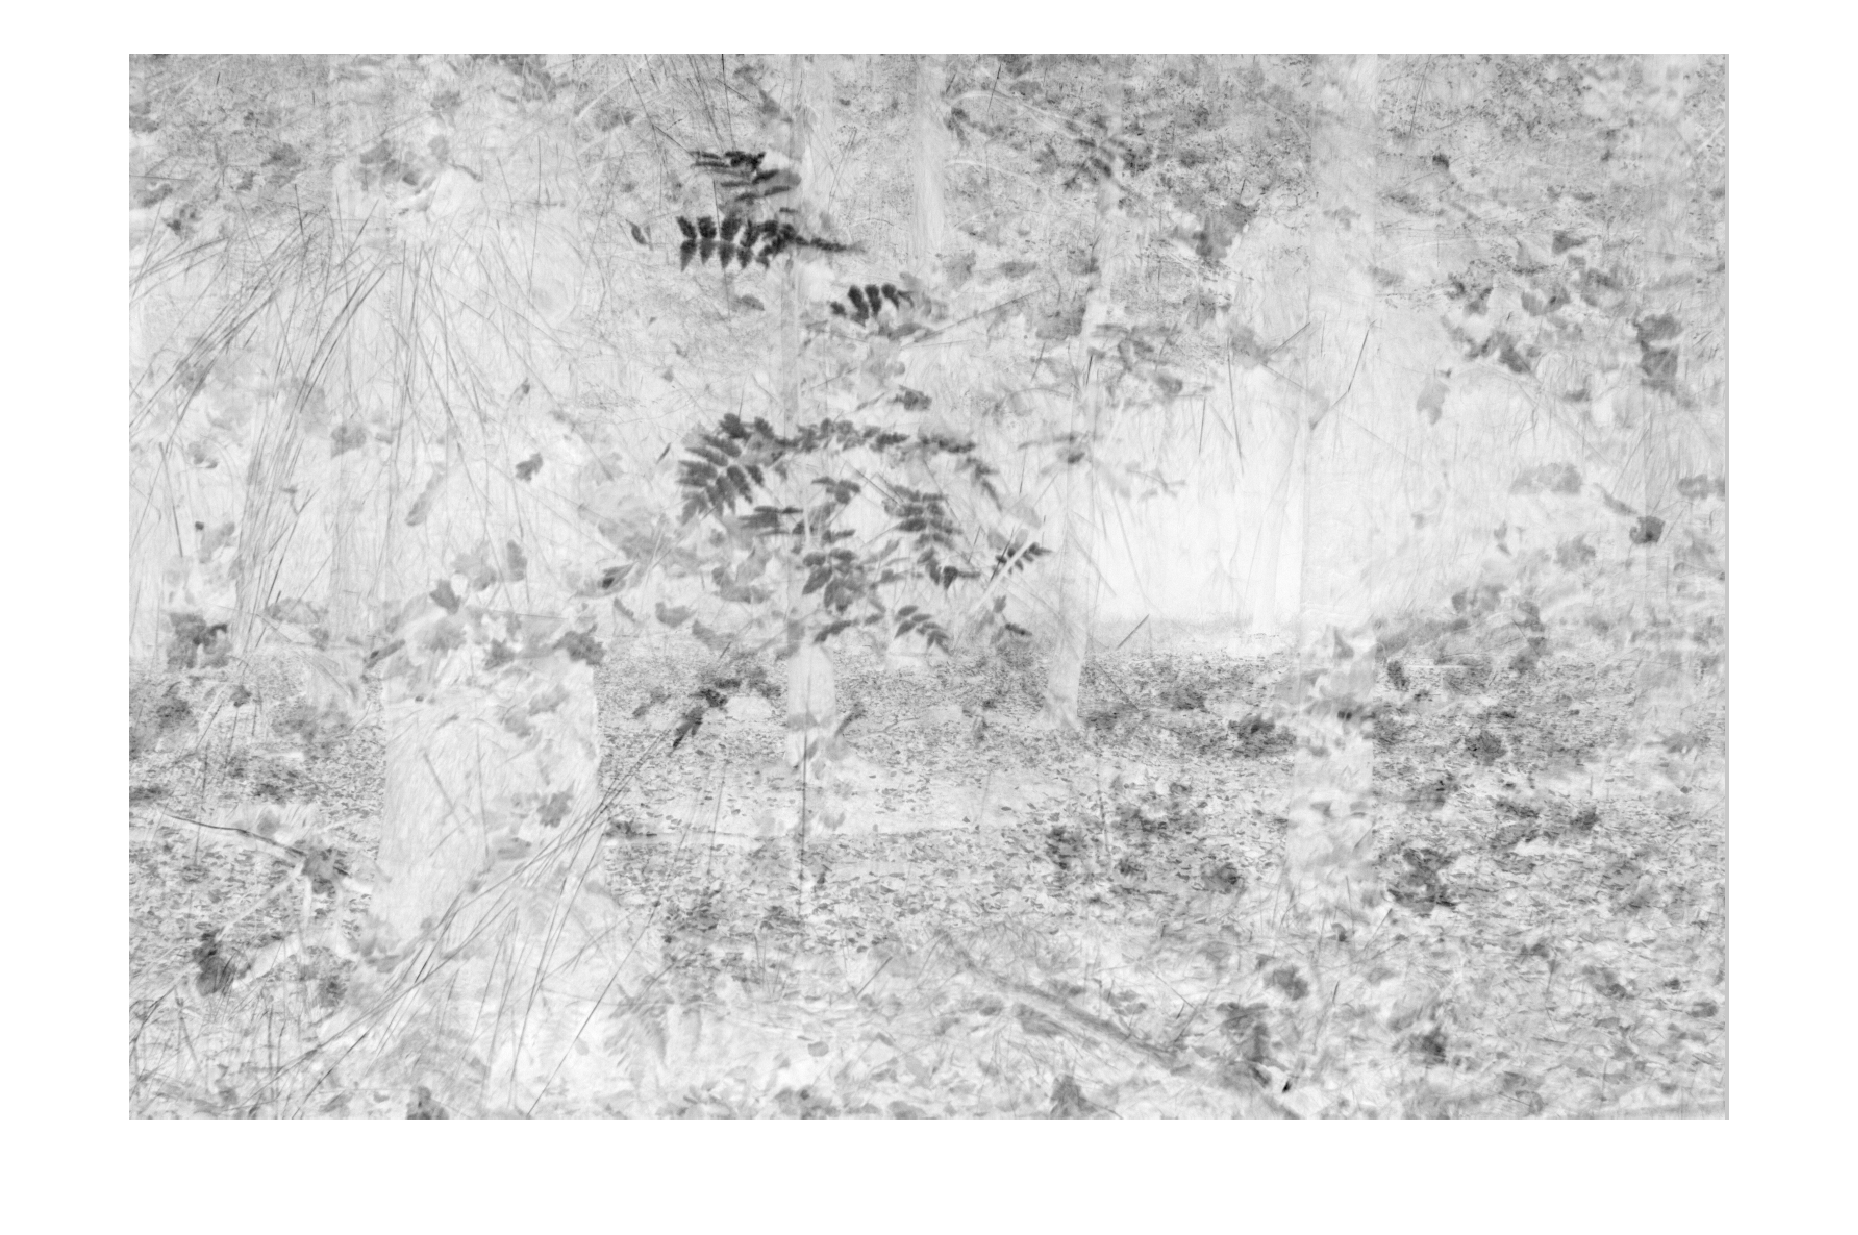
\includegraphics[width=1\textwidth]{Wimg3.eps}
\caption{Whitened Version of Image 3}
\label{fig:Wimg3}
\end{figure}


\subsubsection{Results of ICA}

We then learned a transformation to separate the images using the code that follows:
\lstinputlisting[firstline=57, lastline=65]{problem3code/problem3.m}
This generates the following images, which we can see are better in the case where the whitened data was trained:
\begin{figure}[ht!]
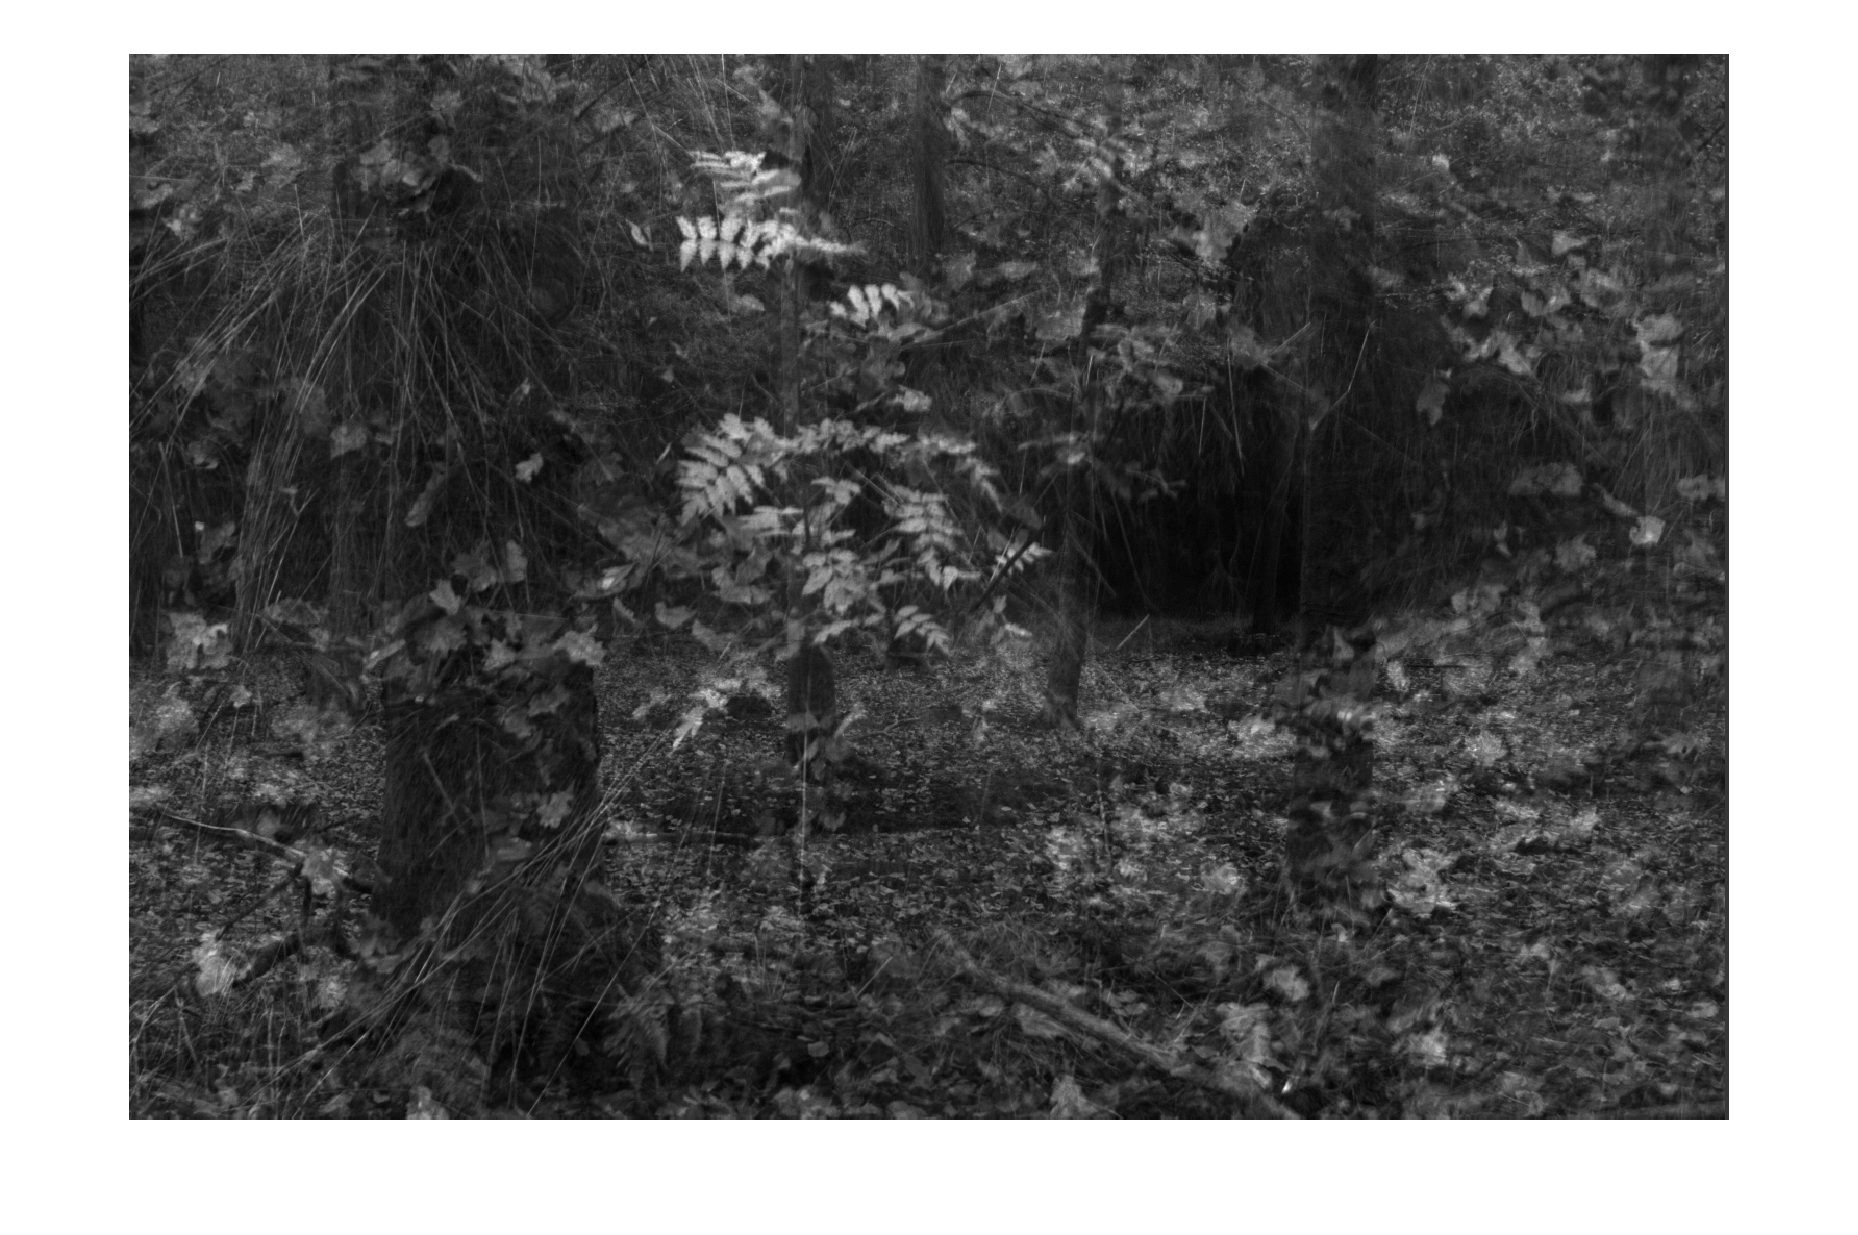
\includegraphics[width=1\textwidth]{Wimg1final.eps}
\caption{ICA of Whitened Image 1}
\label{fig:ICAWimg1}
\end{figure}

\begin{figure}[ht!]
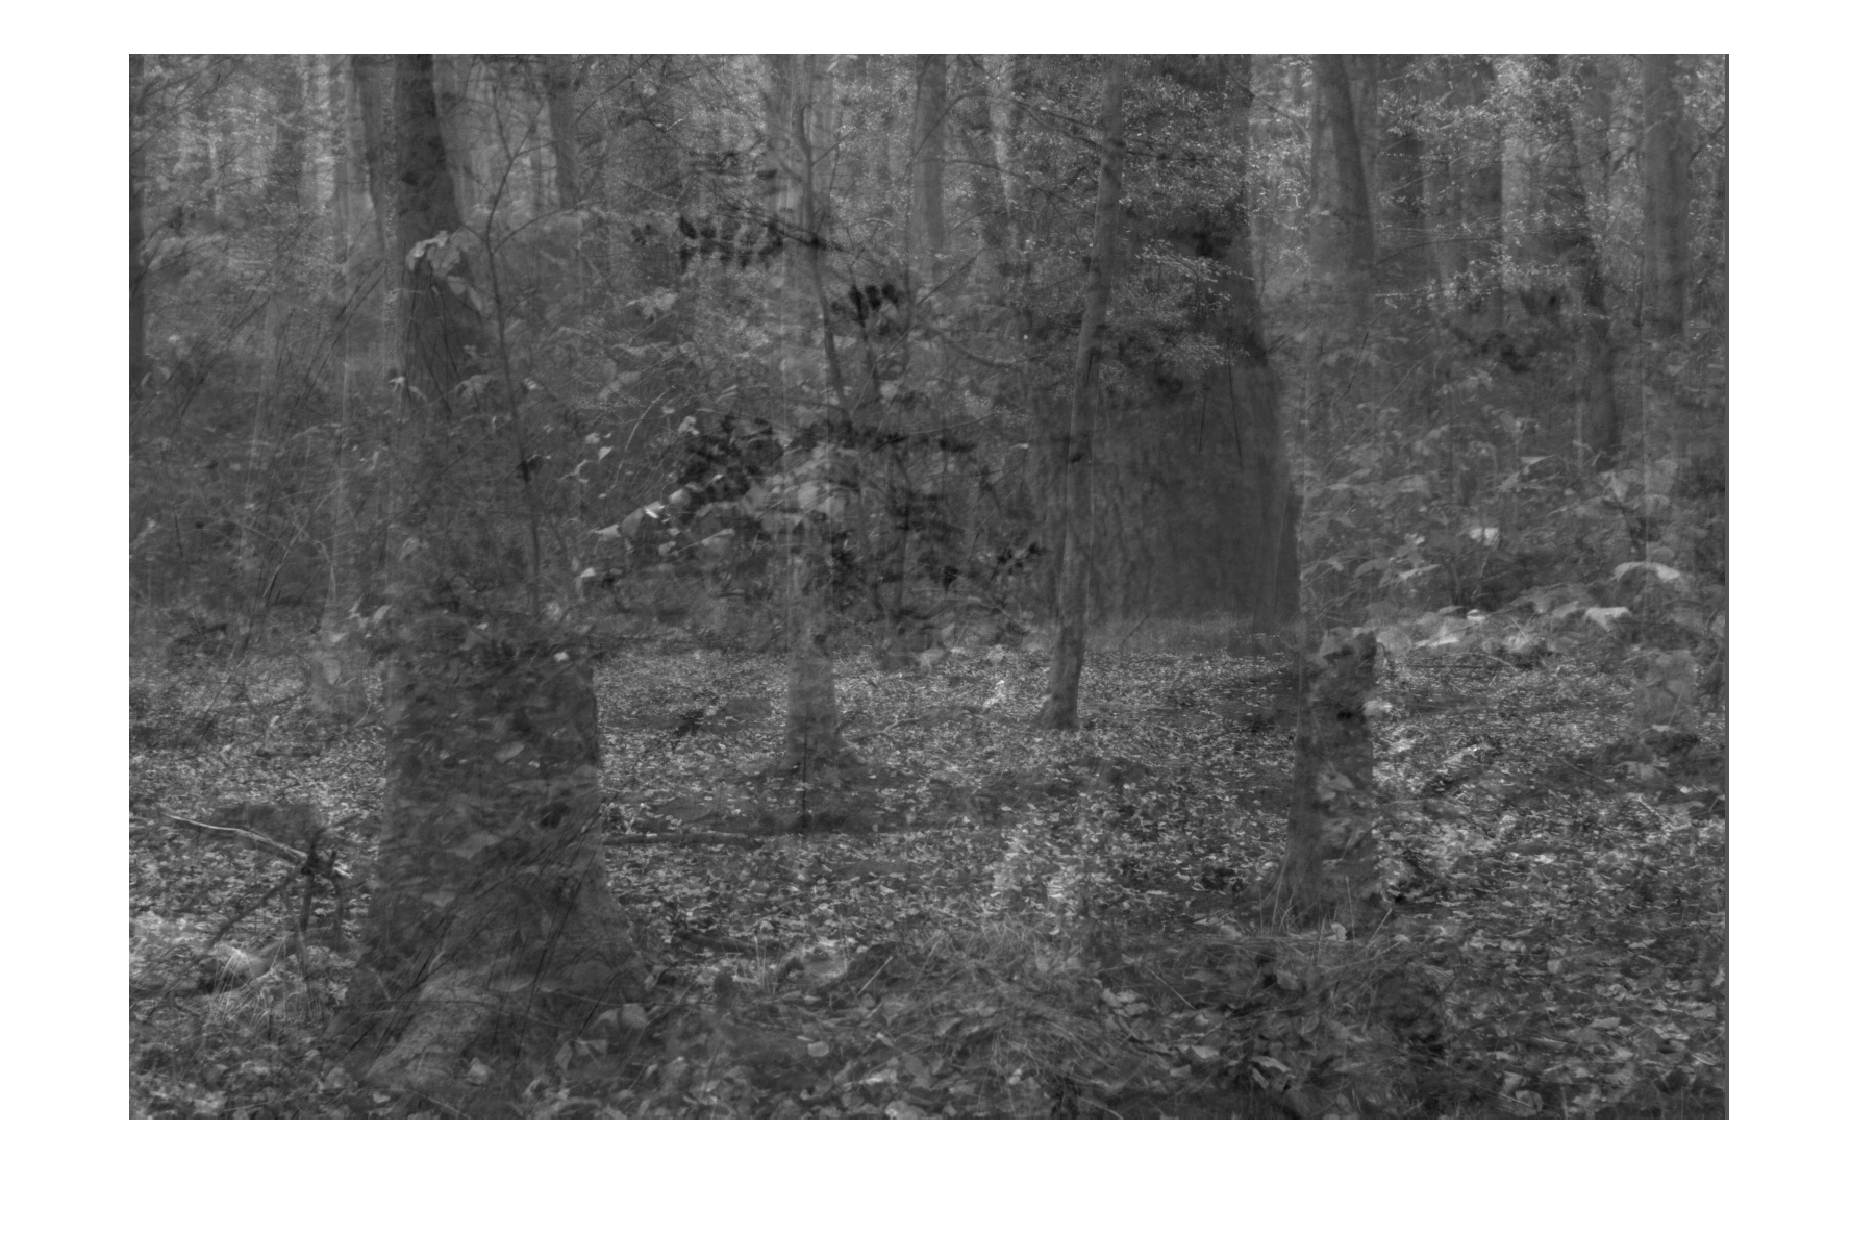
\includegraphics[width=1\textwidth]{Wimg2final.eps}
\caption{ICA of Whitened Image 2}
\label{fig:ICAWimg2}
\end{figure}

\begin{figure}[ht!]
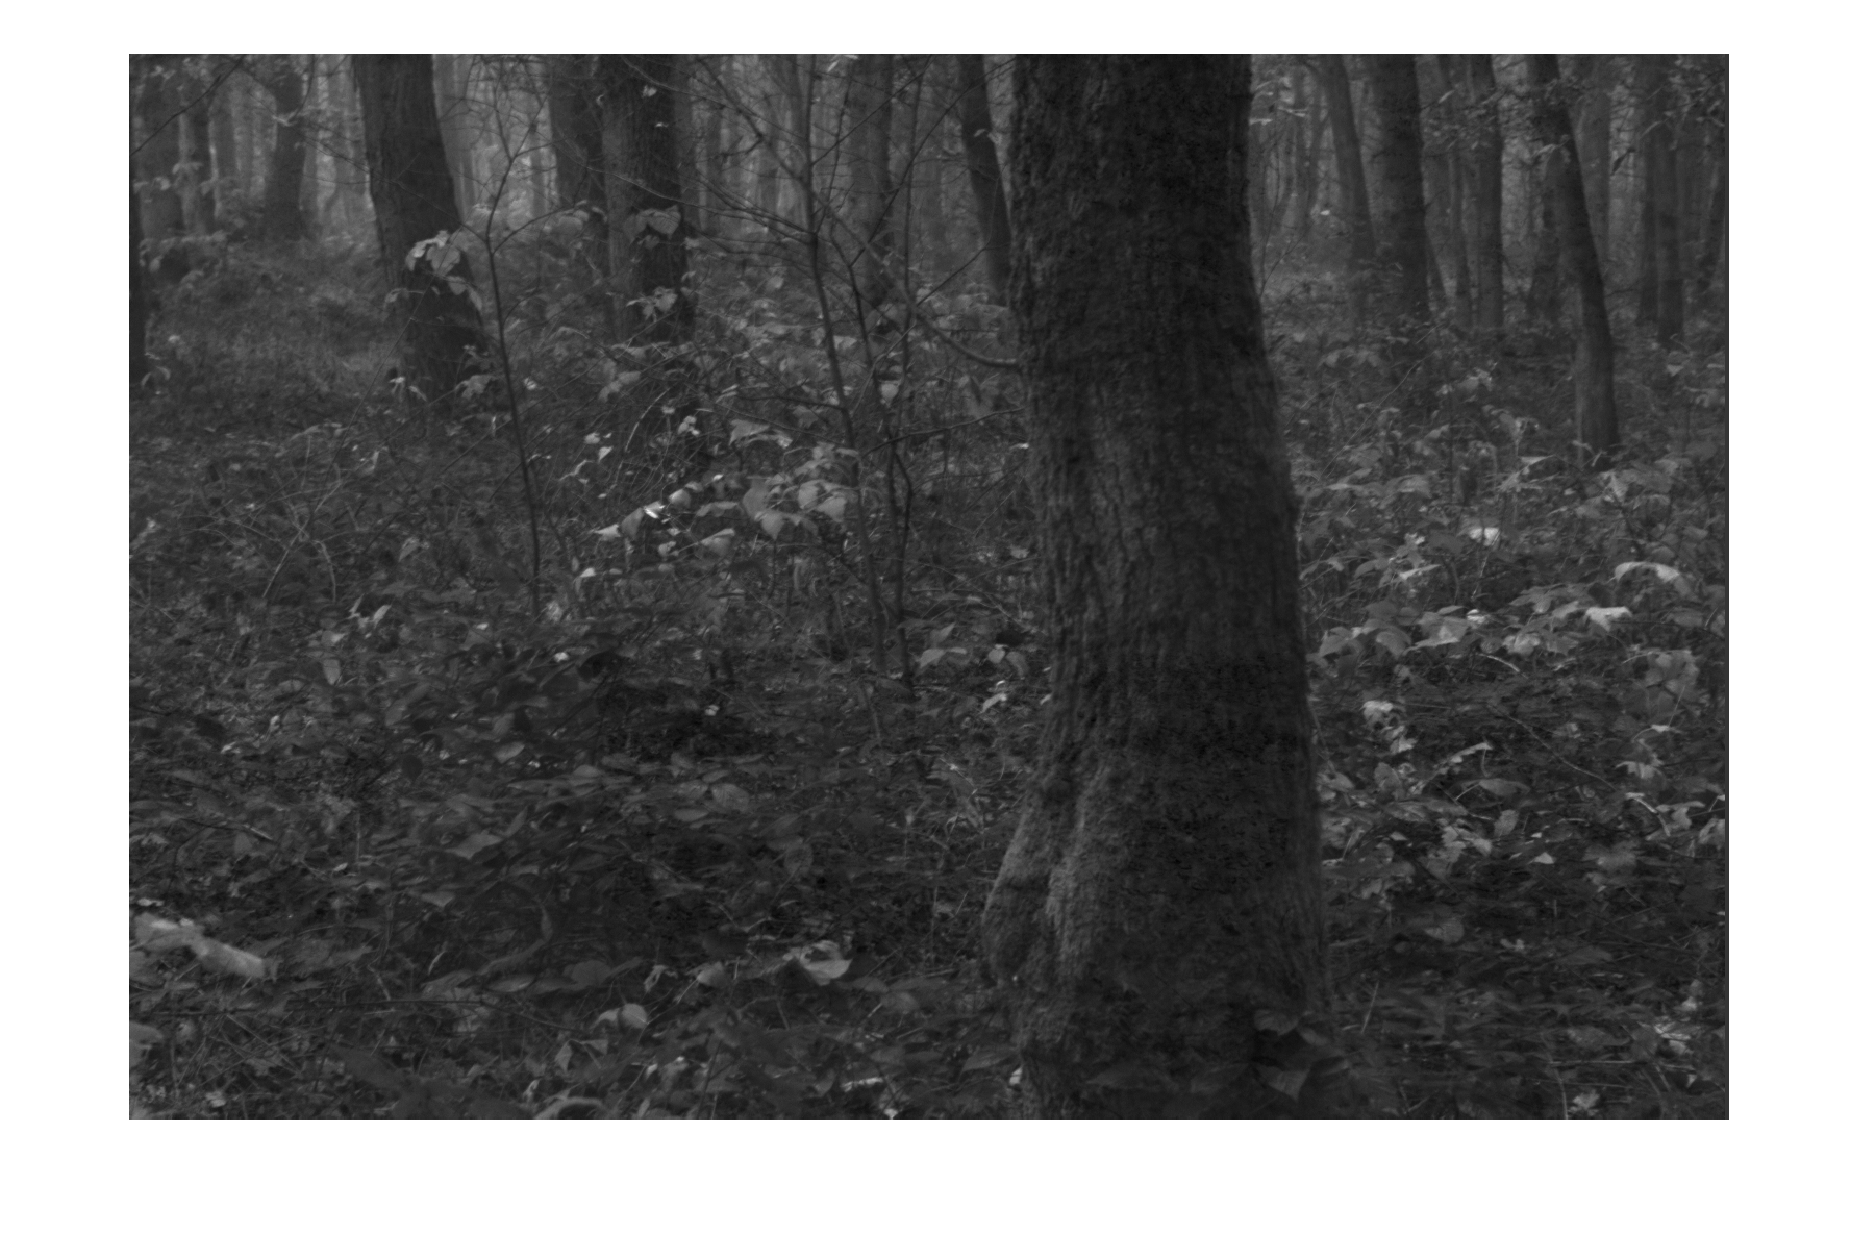
\includegraphics[width=1\textwidth]{Wimg3final.eps}
\caption{ICA of Whitened Image 3}
\label{fig:ICAWimg3}
\end{figure}

\begin{figure}[ht!]
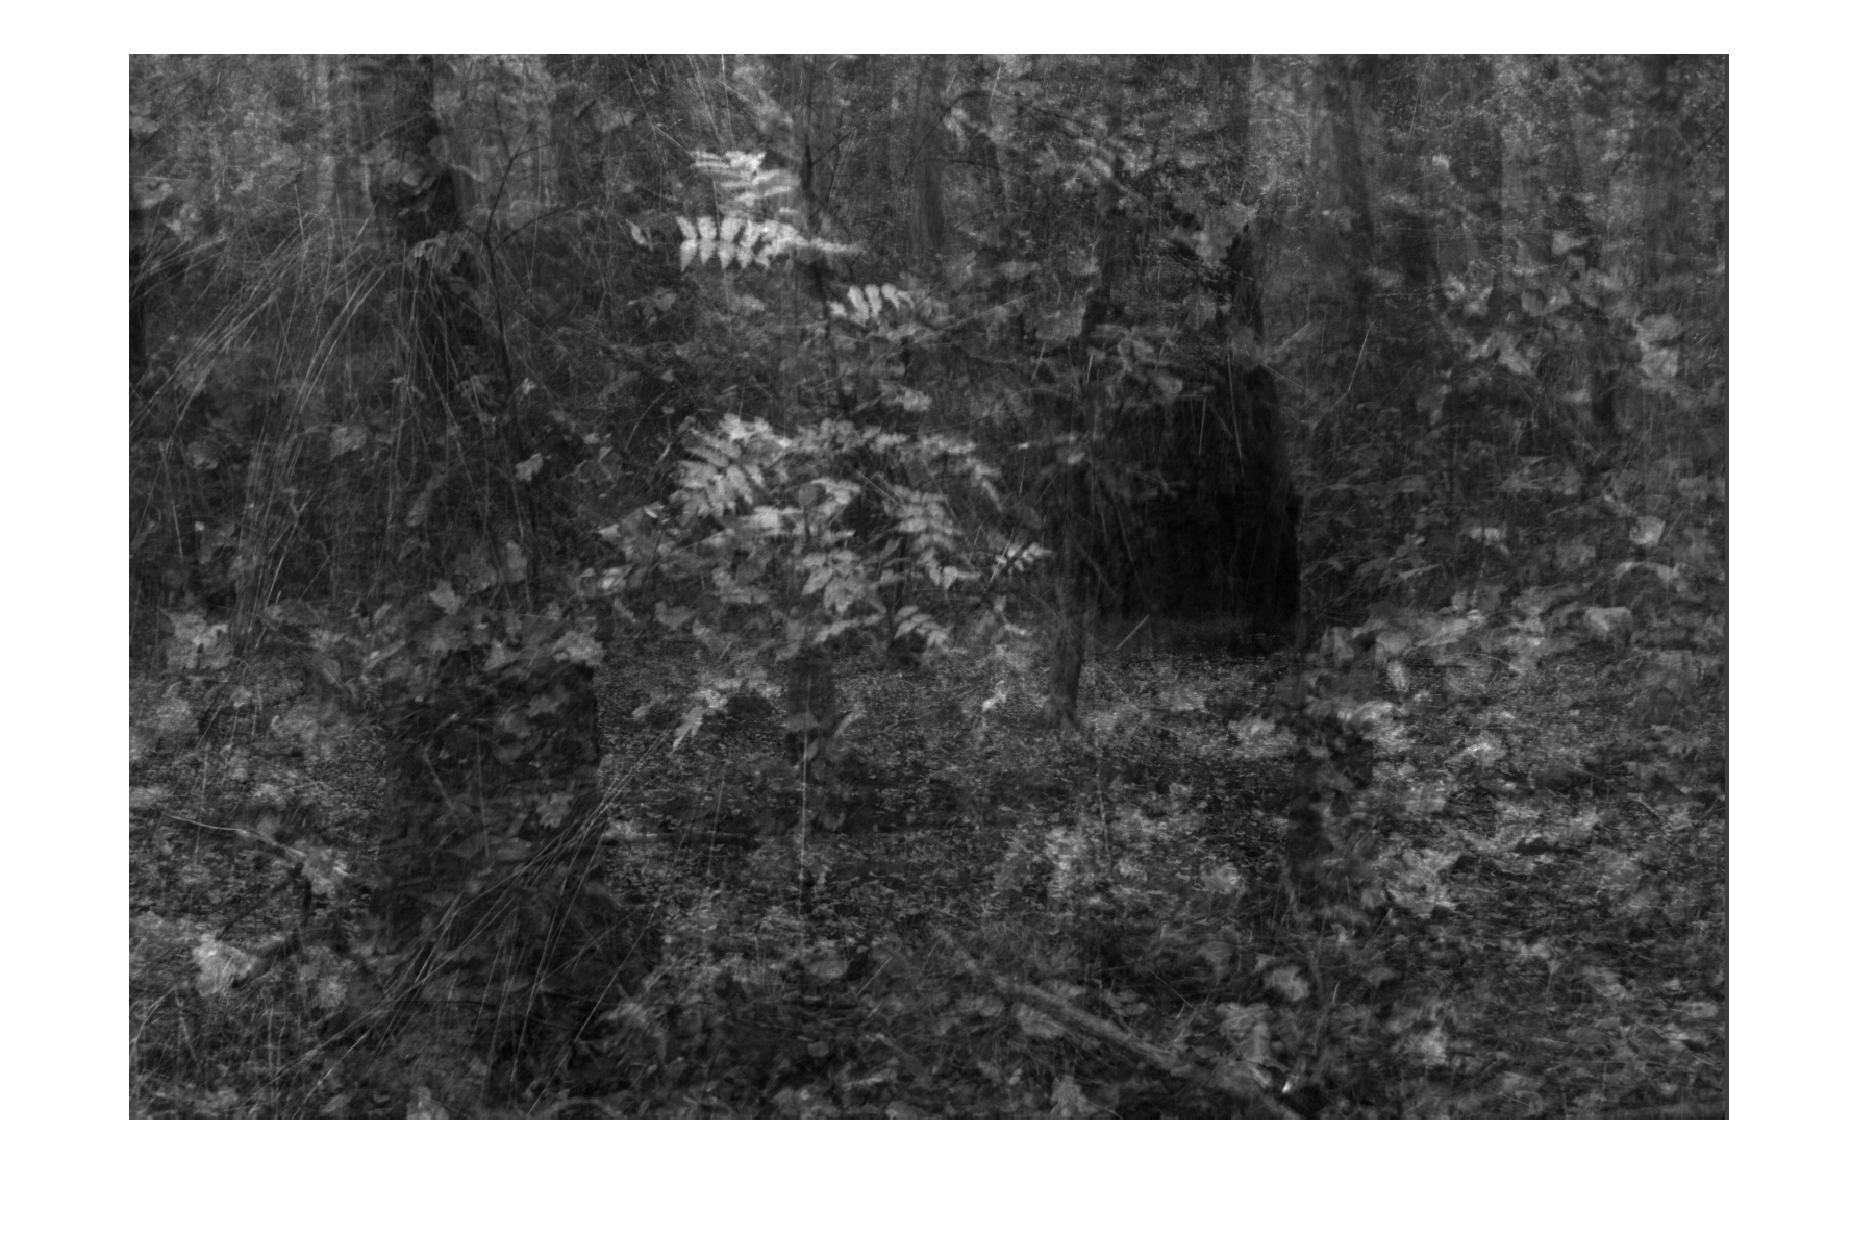
\includegraphics[width=1\textwidth]{img1final.eps}
\caption{ICA of Image 1}
\label{fig:ICAimg1}
\end{figure}

\begin{figure}[ht!]
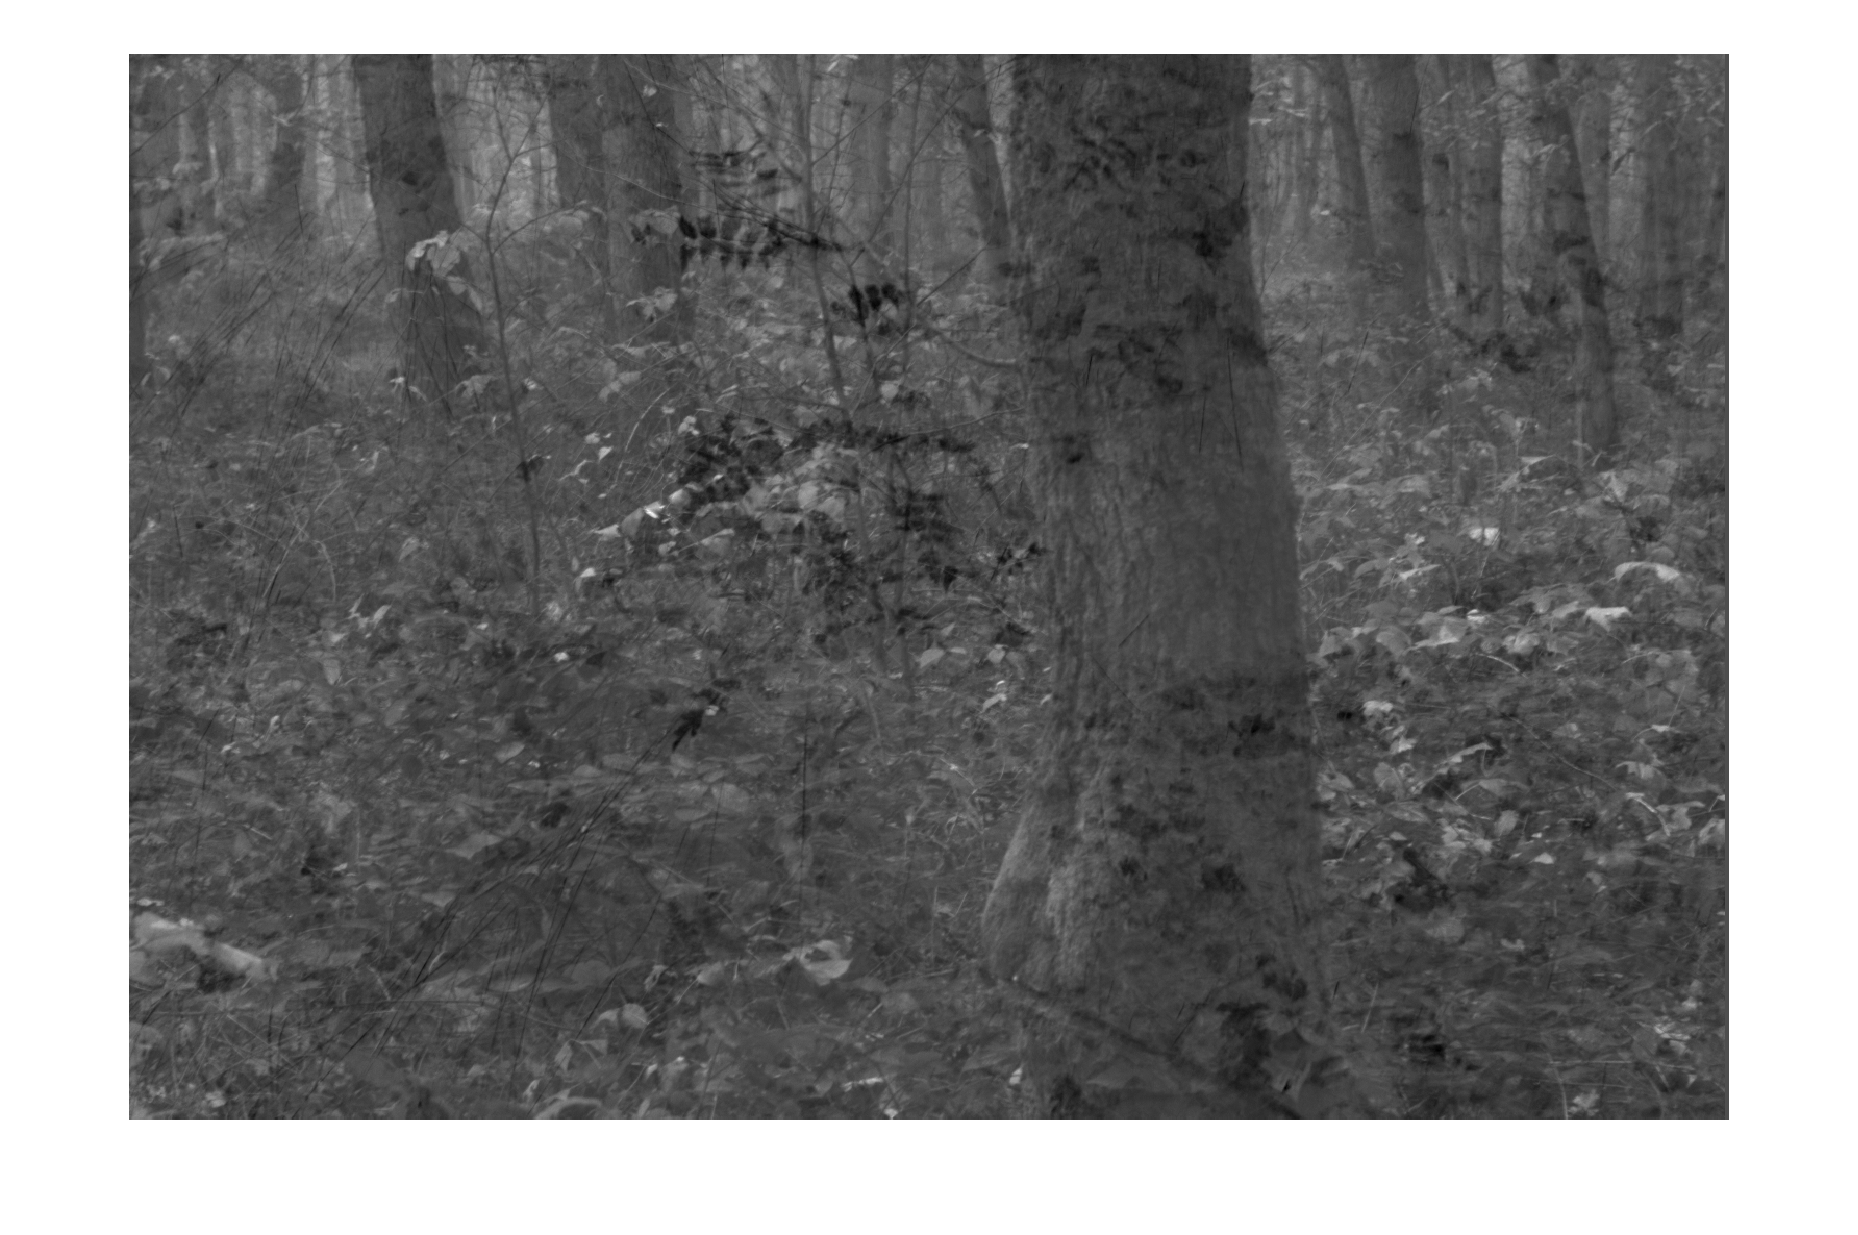
\includegraphics[width=1\textwidth]{img2final.eps}
\caption{ICA of Image 2}
\label{fig:ICAimg2}
\end{figure}

\begin{figure}[ht!]
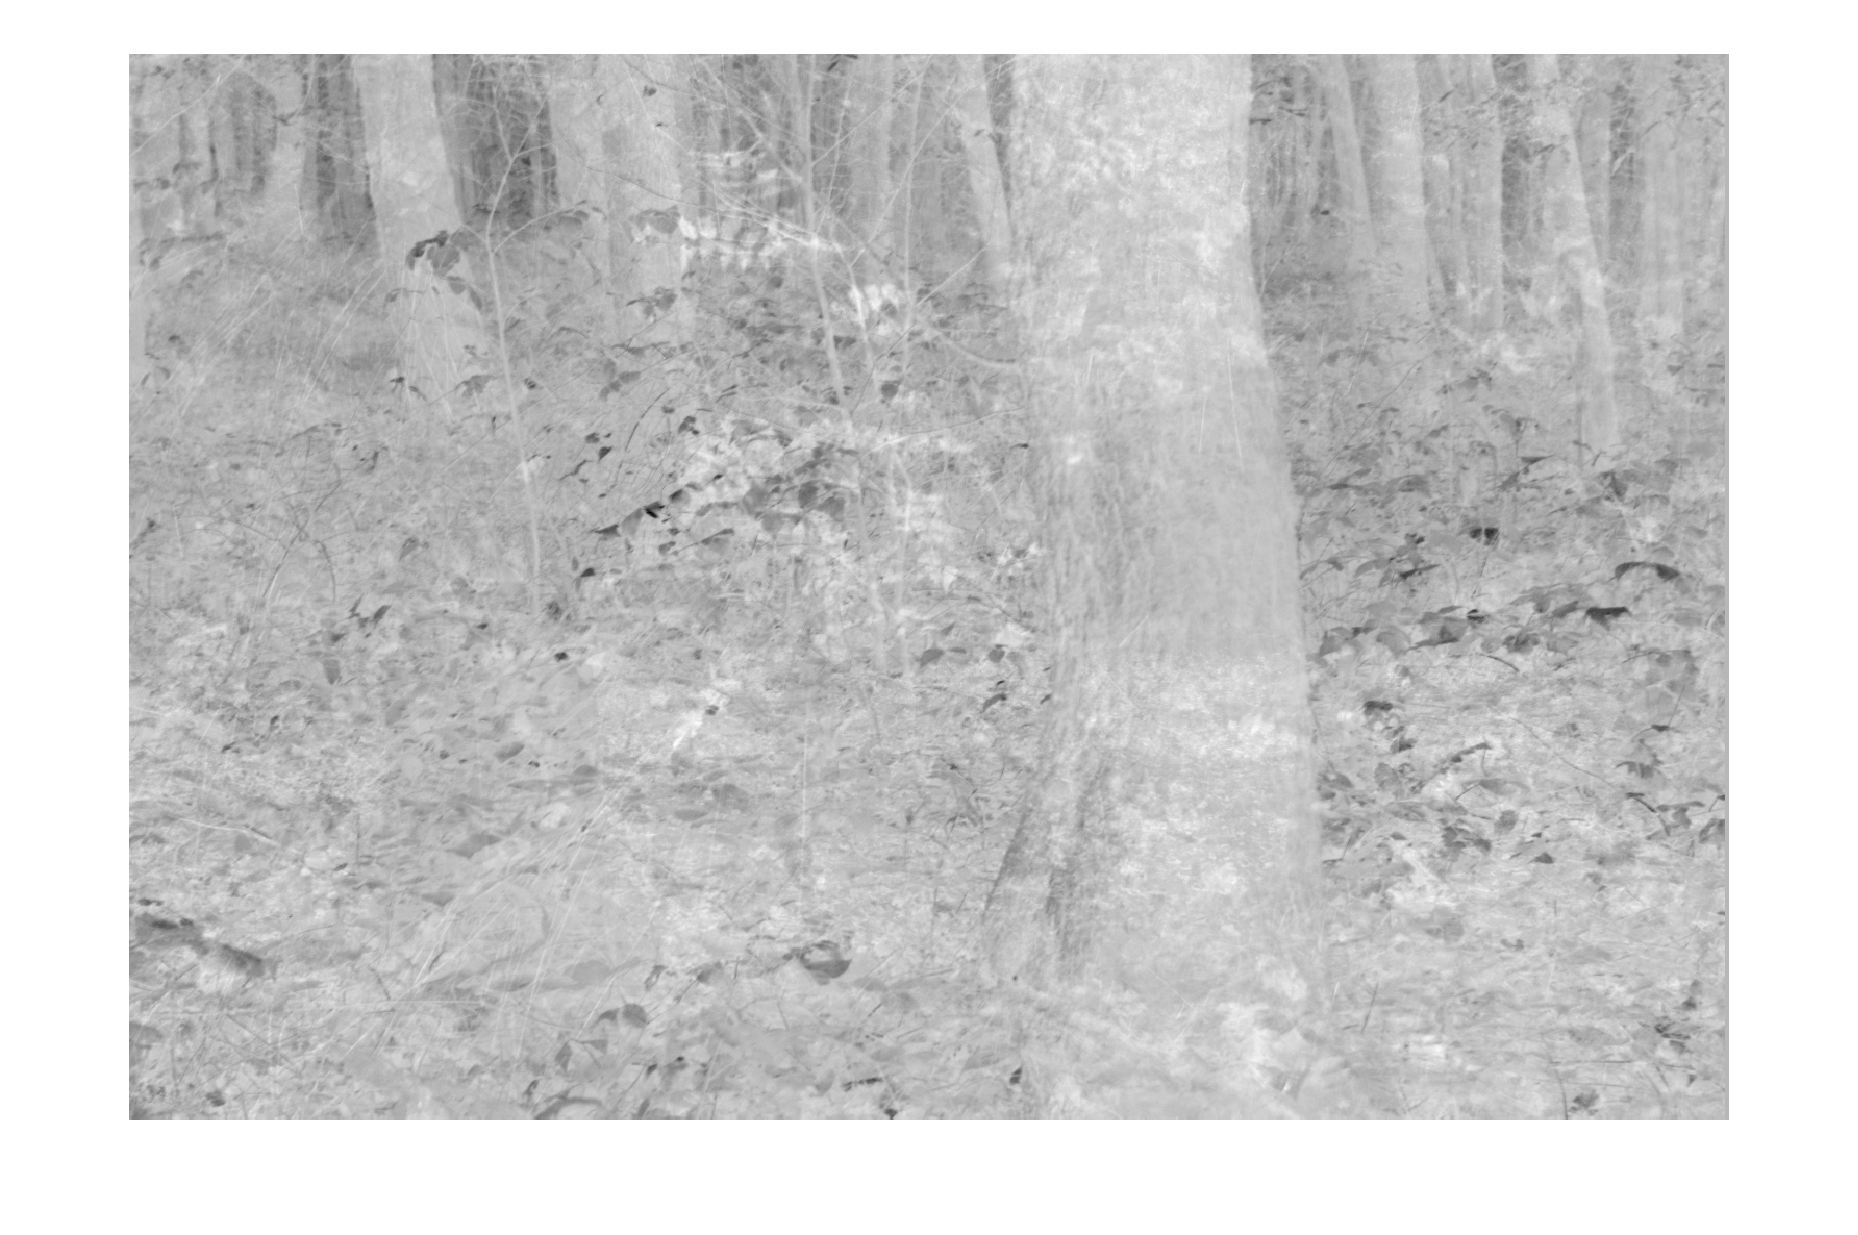
\includegraphics[width=1\textwidth]{img3final.eps}
\caption{ICA of Image 3}
\label{fig:ICAimg3}
\end{figure}


\section{Mathematics of Regression}

This portion of the assignment was submitted separately.



\end{document}
